\documentclass[12pt]{amsart}
\usepackage[T1]{fontenc}
\usepackage[utf8]{inputenc}

\usepackage[top=1.95cm, bottom=1.95cm, left=2.35cm, right=2.35cm]{geometry}


\usepackage{wrapfig}

\usepackage{hyperref}
\usepackage{enumitem}
\usepackage{tcolorbox}
\usepackage{float}
\usepackage{cleveref}
\usepackage{multicol}
\usepackage{fancyvrb}
\usepackage{enumitem}
\usepackage{amsmath}
\usepackage{textcomp}
\usepackage[french]{babel}
\frenchsetup{StandardItemLabels=true}
\usepackage[
    type={CC},
    modifier={by-nc-sa},
	version={4.0},
]{doclicense}

\usepackage{tnsmath}

\DeclareMathOperator{\taille}{\tau}

\newtheorem{defi}{Définition}
\newtheorem{fact}{Fait}
\newtheorem*{proof*}{Preuve}

\newtheorem{remark}{Remarque}[section]

\NewDocumentCommand{\area}{m}{\mathrm{Aire}(#1)}
\NewDocumentCommand{\perim}{m}{\mathrm{Perim}(#1)}
\NewDocumentCommand{\degreg}{m}{\mathrm{dreg}(#1)}

\setlength\parindent{0pt}


\begin{document}

\title{BROUILLON - Inégalités isopérimétriques restreintes à la géométrie}
\author{Christophe BAL}
\date{18 Jan. 2025 -- 22 Jan. 2025}
\maketitle


\begin{center}
	\hrule\vspace{.3em}
	{
		\fontsize{1.35em}{1em}\selectfont
		\textbf{Mentions \og légales \fg}
	}
			
	\vspace{0.45em}
	\doclicenseThis
	\hrule
\end{center}



\setcounter{tocdepth}{2}
\tableofcontents


% ------------- %


\newpage

%Ce document s'intéresse au classique problème de l'isopérimétrie plane, c'est-à-dire la recherche d'une surface plane maximisant son aire pour un périmètre fixé.
%Nous allons nous restreindre au cas élémentaire des polygones, tout en nous limitant à des preuves purement géométriques. La restriction est donc double, voire triple une fois les différentes démonstrations lues.
%
%
%\begin{tcolorbox}
%	\itshape\small
%	Pour ne pas alourdir le texte, on raisonnera modulo des isométries, positives ou non. Ainsi, on pourra parler \og \emph{du carré équilatéral de côté $c$} \fg\,, \og \emph{du triangle équilatéral de côté $c$} \fg...
%	Indiquons aussi que le niveau de lecture de ce document, hors remarques, se veut très élémentaire.
%\end{tcolorbox}
%
%
%% ------------- %
%
%
%\section{Les rectangles}
%
%\begin{fact} \label{iso-rect}
	Considérons tous les rectangles de périmètre fixé $p$. Parmi tous ces rectangles, celui d'aire maximale est le carré de côté $c = \num{.25} p$.
\end{fact}


\begin{proof}
	Une preuve courante est d'exprimer l'aire du rectangle comme un polynôme du 2\ieme\ degré en $L$ par exemple.%
	\footnote{
		L'aire est donnée par $L \ell = L (\num{.5} p - L)$ qui est maximale en $L_M = \num{.25} p$ (moyenne des racines), d'où $\ell_M = \num{.25} p = L_M$.
	}
	On peut en fait faire plus simplement grâce au dessin suivant où les rectangles $1$, $2$ et $3$ sont isométriques au rectangle vert étudié de dimension $L \times \ell$.

	\begin{center}
		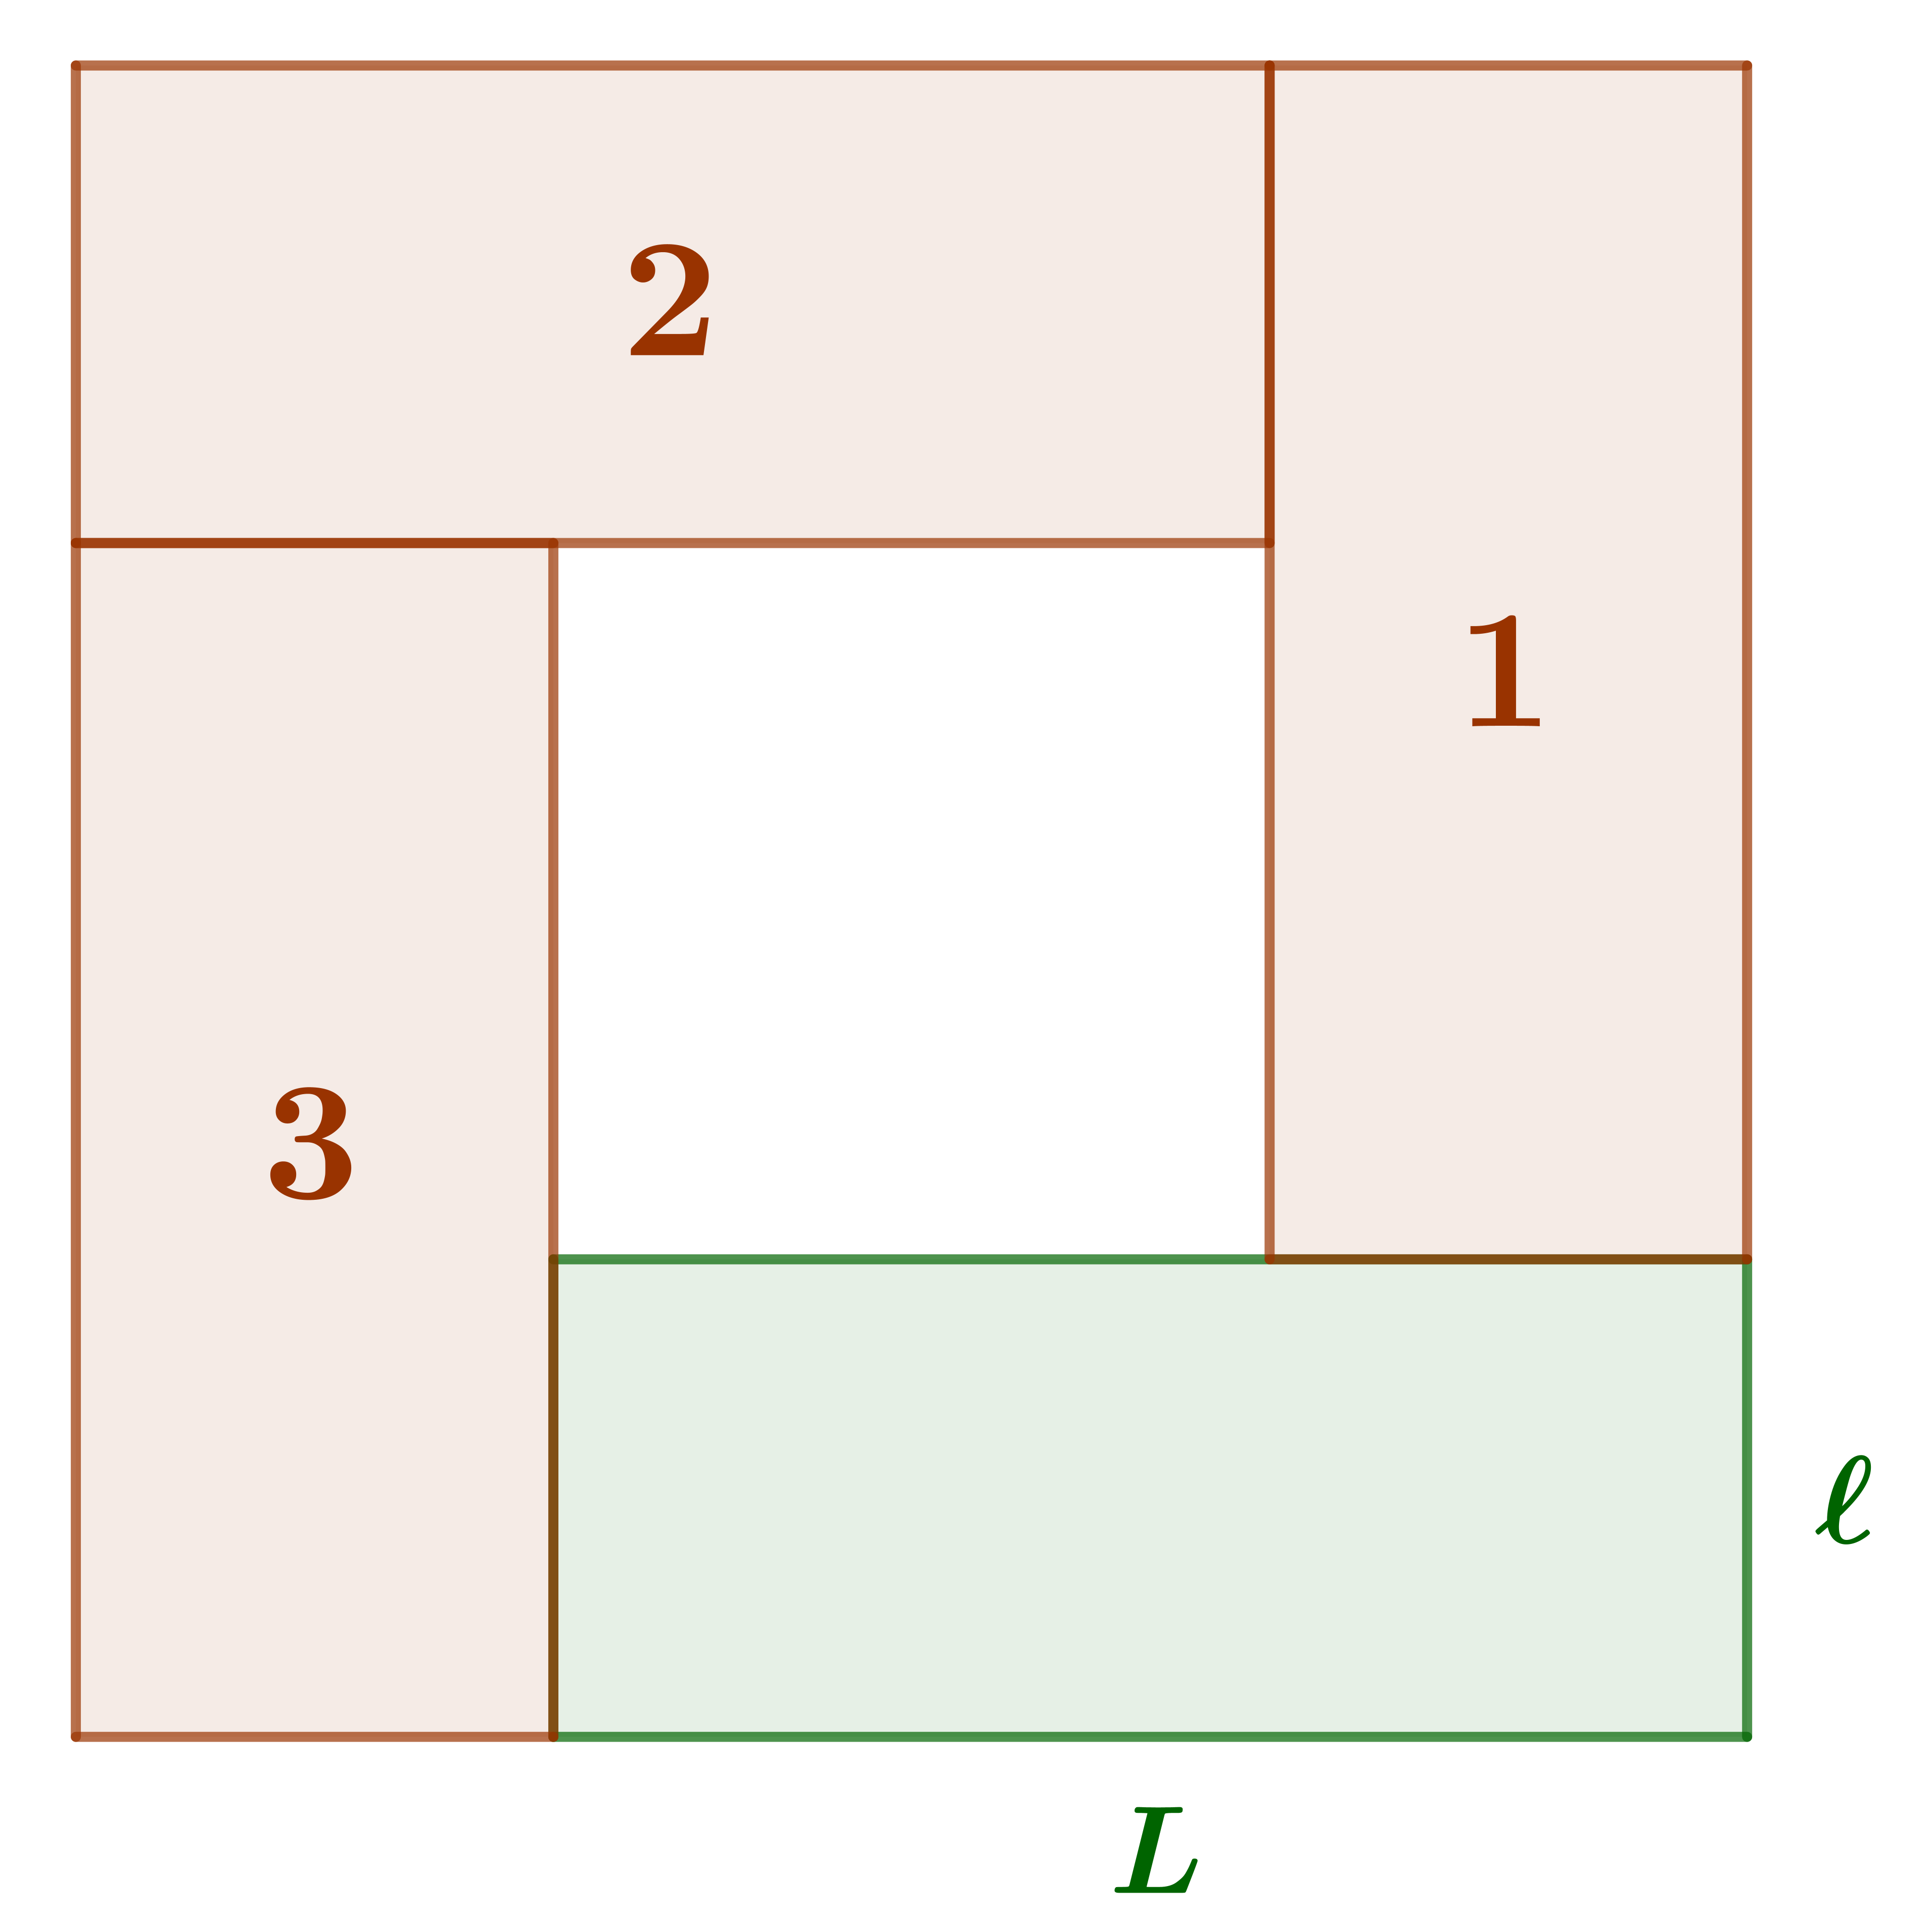
\includegraphics[scale=.4]{content/rectangle/rectangle.png}
	\end{center}
	
	Le raisonnement tient alors aux constations suivantes accessibles à un collégien.
	%
	\begin{enumerate}
		\item Le grand carré a une aire supérieure ou égale à $4 L \ell$.

		\item Le grand carré a un périmètre égal à $4 (L + \ell)$.

		\item Via une homothétie de rapport \num{.5}\,, nous obtenons un carré d'aire supérieure ou égale à $\num{.5}^2 \times 4 L \ell =  L \ell$, et de périmètre égal à $\num{.5} \times 4 (L + \ell) = 2 (L + \ell)$.
	\end{enumerate}
	
	Donc pour tout rectangle de périmètre $p = 2 (L + \ell)$ et d'aire $L \ell$, nous pouvons construire un carré de périmètre identique, mais avec une aire supérieure ou égale à  $L \ell$. Joli! Non?
\end{proof}


\begin{remark}
	Au passage, nous avons pour $(L ; \ell) \in \big( \RRsp \big)^2$, $4 L \ell \leq (L + \ell)^2$, c'est-à-dire $2 L \ell \leq L^2 + \ell^2$, d'où $\sqrt{L \ell} \leq \sqrt{\frac12 (L^2 + \ell^2)}$, soit la comparaison des moyennes géométriques et quadratiques d'ordre $2$.
\end{remark}

%
%
% ------------- %
%
%
%\section{Les parallélogrammes}
%
%\begin{fact} \label{iso-para}
	Considérons tous les parallélogrammes de périmètre fixé $p$. Parmi tous ces parallélogrammes, un seul est d'aire maximale, c'est le carré de côté $c = \num{.25} p$.
\end{fact}


\begin{proof}
	Le calcul de l'aire d'un parallélogramme, voir le dessin ci-dessous, nous donne 
	$\area{ABCD} = \area{ABHH^{\,\prime}}$ et 
	$\perim{ABCD} \geq \perim{ABHH^{\,\prime}}$, 
	avec égalité uniquement si $ABCD$ est un rectangle. 
	
	\begin{center}
		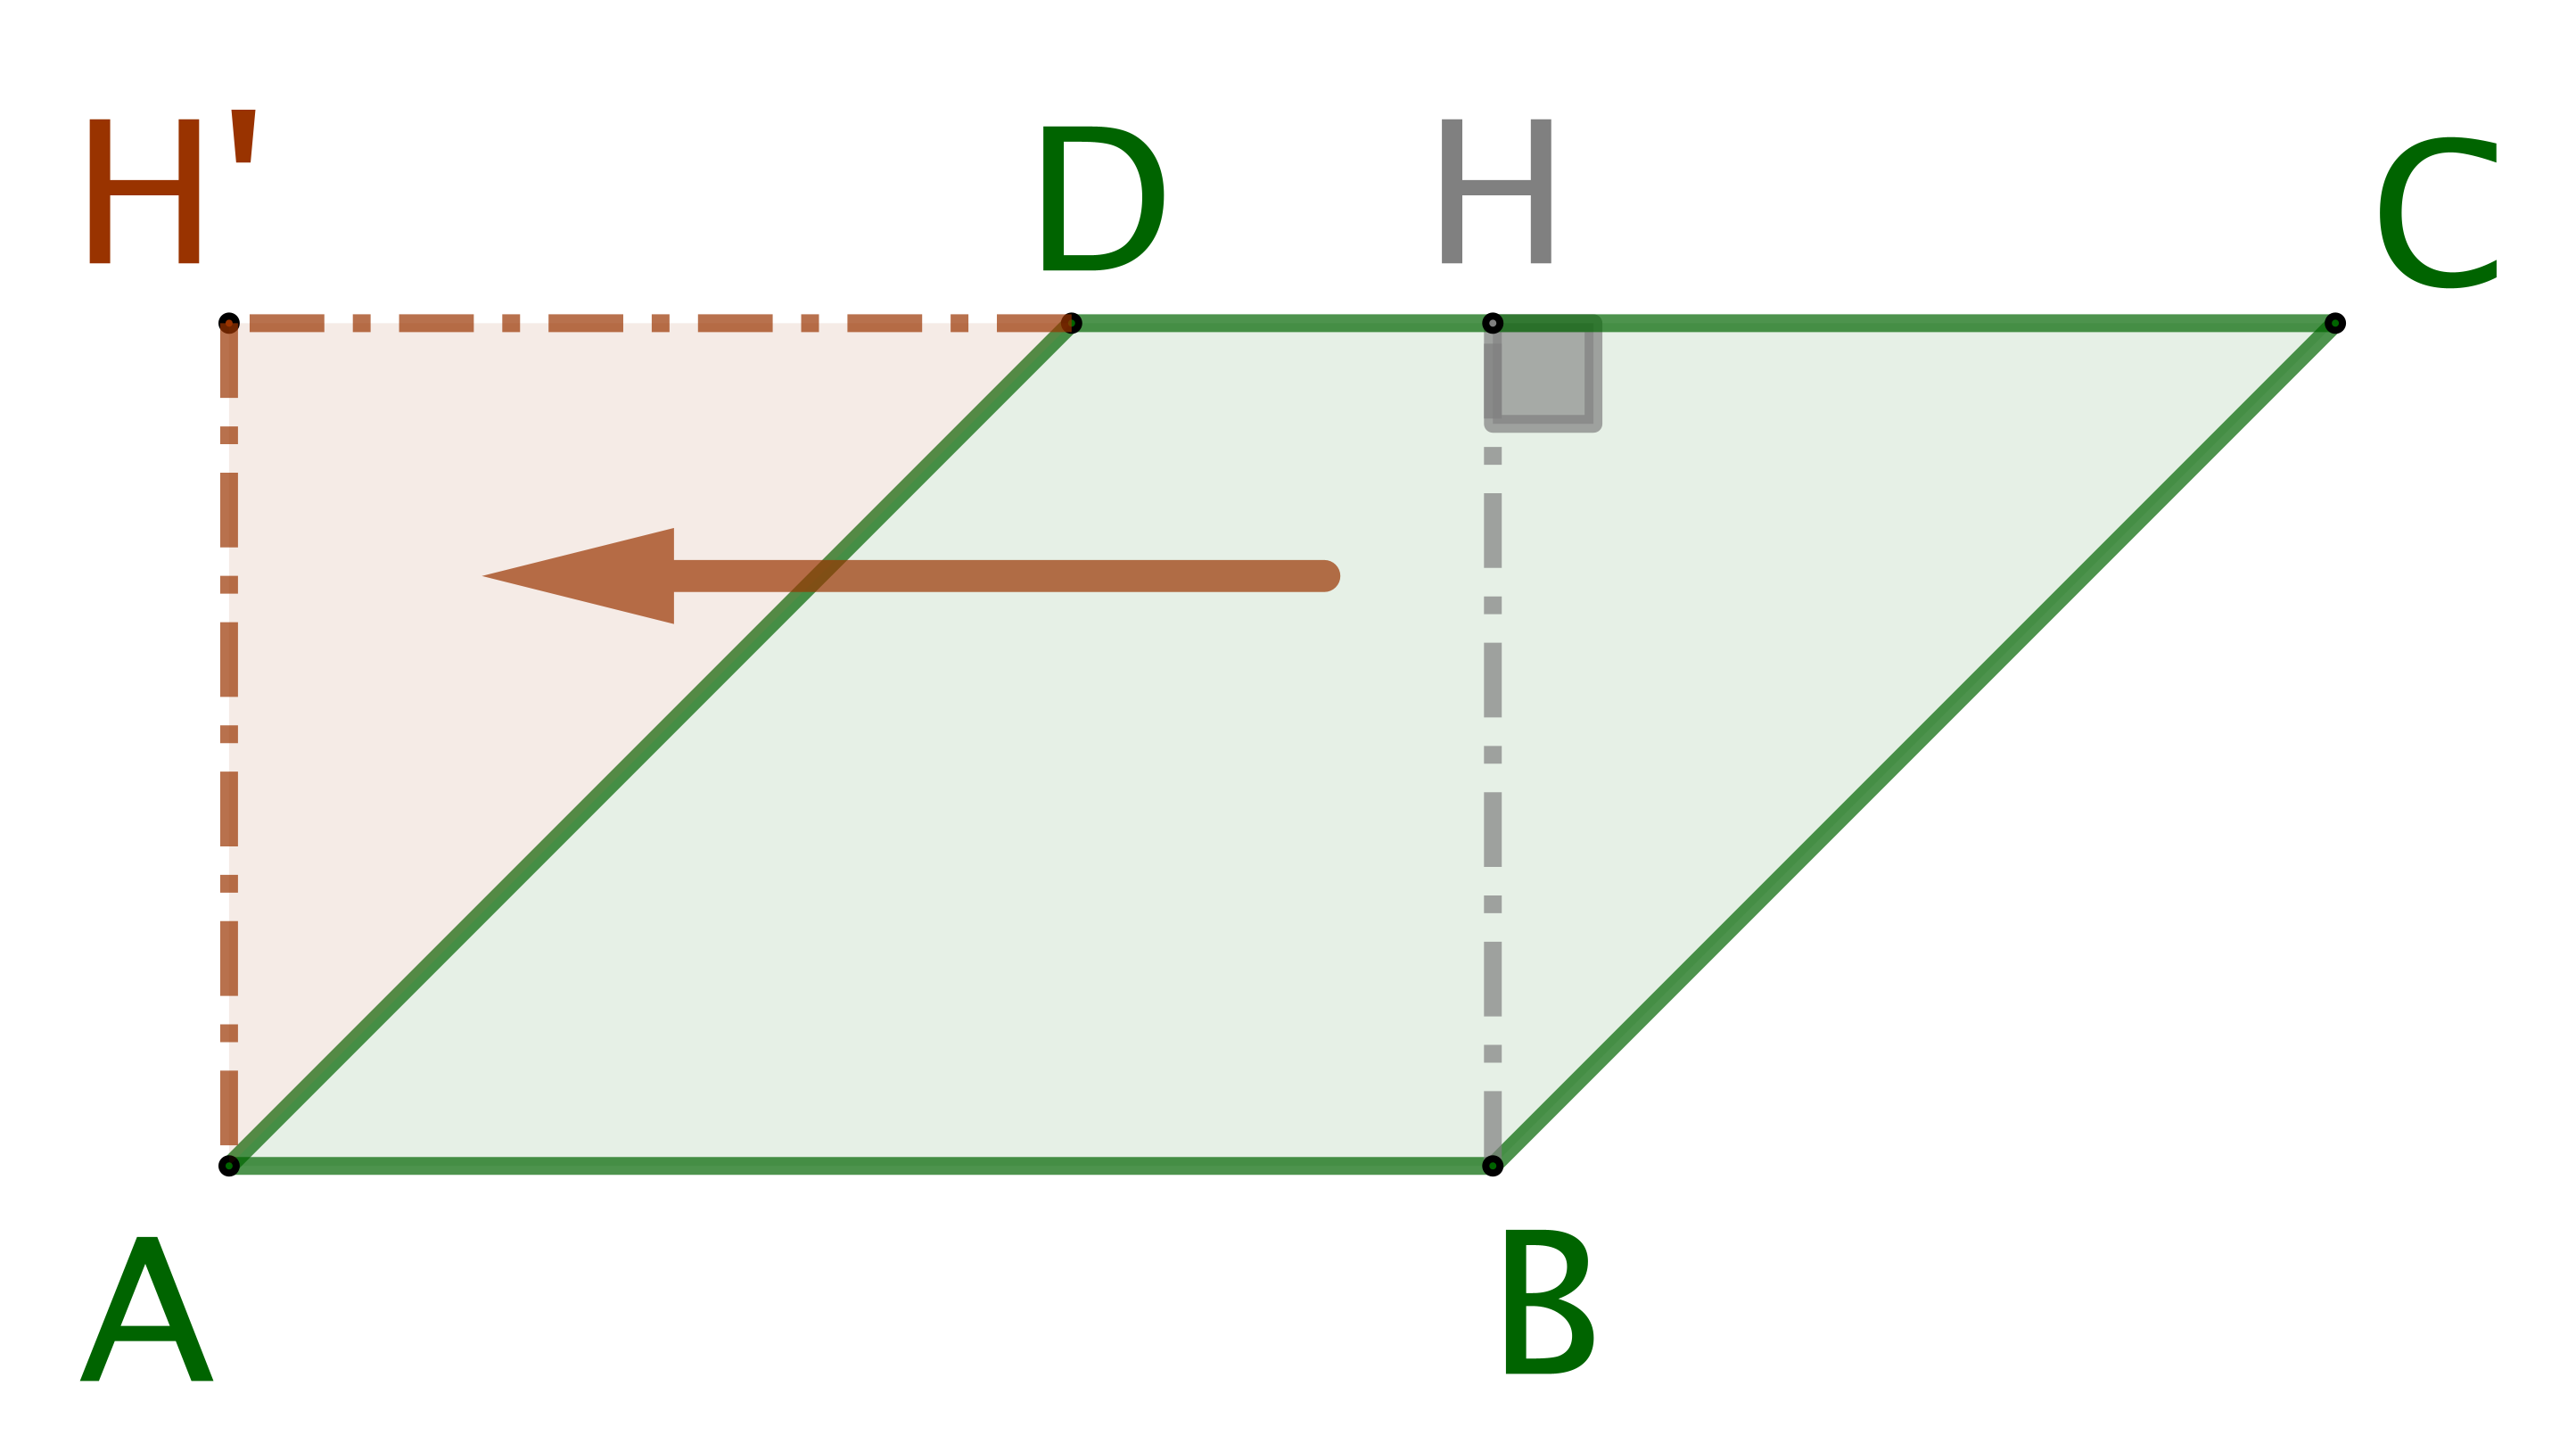
\includegraphics[scale=.4]{content/parallelogram/para-2-rect.png}
	\end{center}
	
	Via une homothétie de rapport $r = \frac{\perim{ABCD}}{\perim{ABHH^{\,\prime}}} \geq 1$, nous obtenons un rectangle 
	de périmètre égal à $p$,
	et d'aire supérieure ou égale à $\area{ABCD}$, 
	avec égalité uniquement si $ABCD$ est un rectangle.
	Nous revenons à la situation du fait \ref{iso-rect} qui permet de conclure très facilement.
\end{proof}


% ----------------------- %


\begin{remark}
	Une méthode analytique devient pénible ici, car il faut, par exemple, prendre en compte l'angle au sommet $A$ du parallélogramme. L'auteur préfère battre en retraite en clôturant cette remarque ici.
%	\footnote{
%		Et oui, l'auteur est un lâche.
%	}
\end{remark}

%
%
%% ------------- %
%
%
%\section{Les triangles avec un côté fixé}
%
%\begin{fact} \label{tri-one-side-fixed}
	Considérons tous les triangles de périmètre fixé, et ayant tous un côté en commun.
	Parmi tous ces triangles, il en existe un seul d'aire maximale, c'est le triangle isocèle ayant pour base le côté commun.
\end{fact}


\begin{proof}
	Soit $ABC$ un triangle de périmètre $p$, et fixons le côté $[AB]$. 
	Pour tout point $M$ sur la parallèle à $(AB)$ passant par $C$, nous savons que $\area{ABM} = \area{ABC}$. Notons alors $O$ le point sur cette parallèle tel que $ABO$ soit isocèle en $O$.

	\begin{center}
		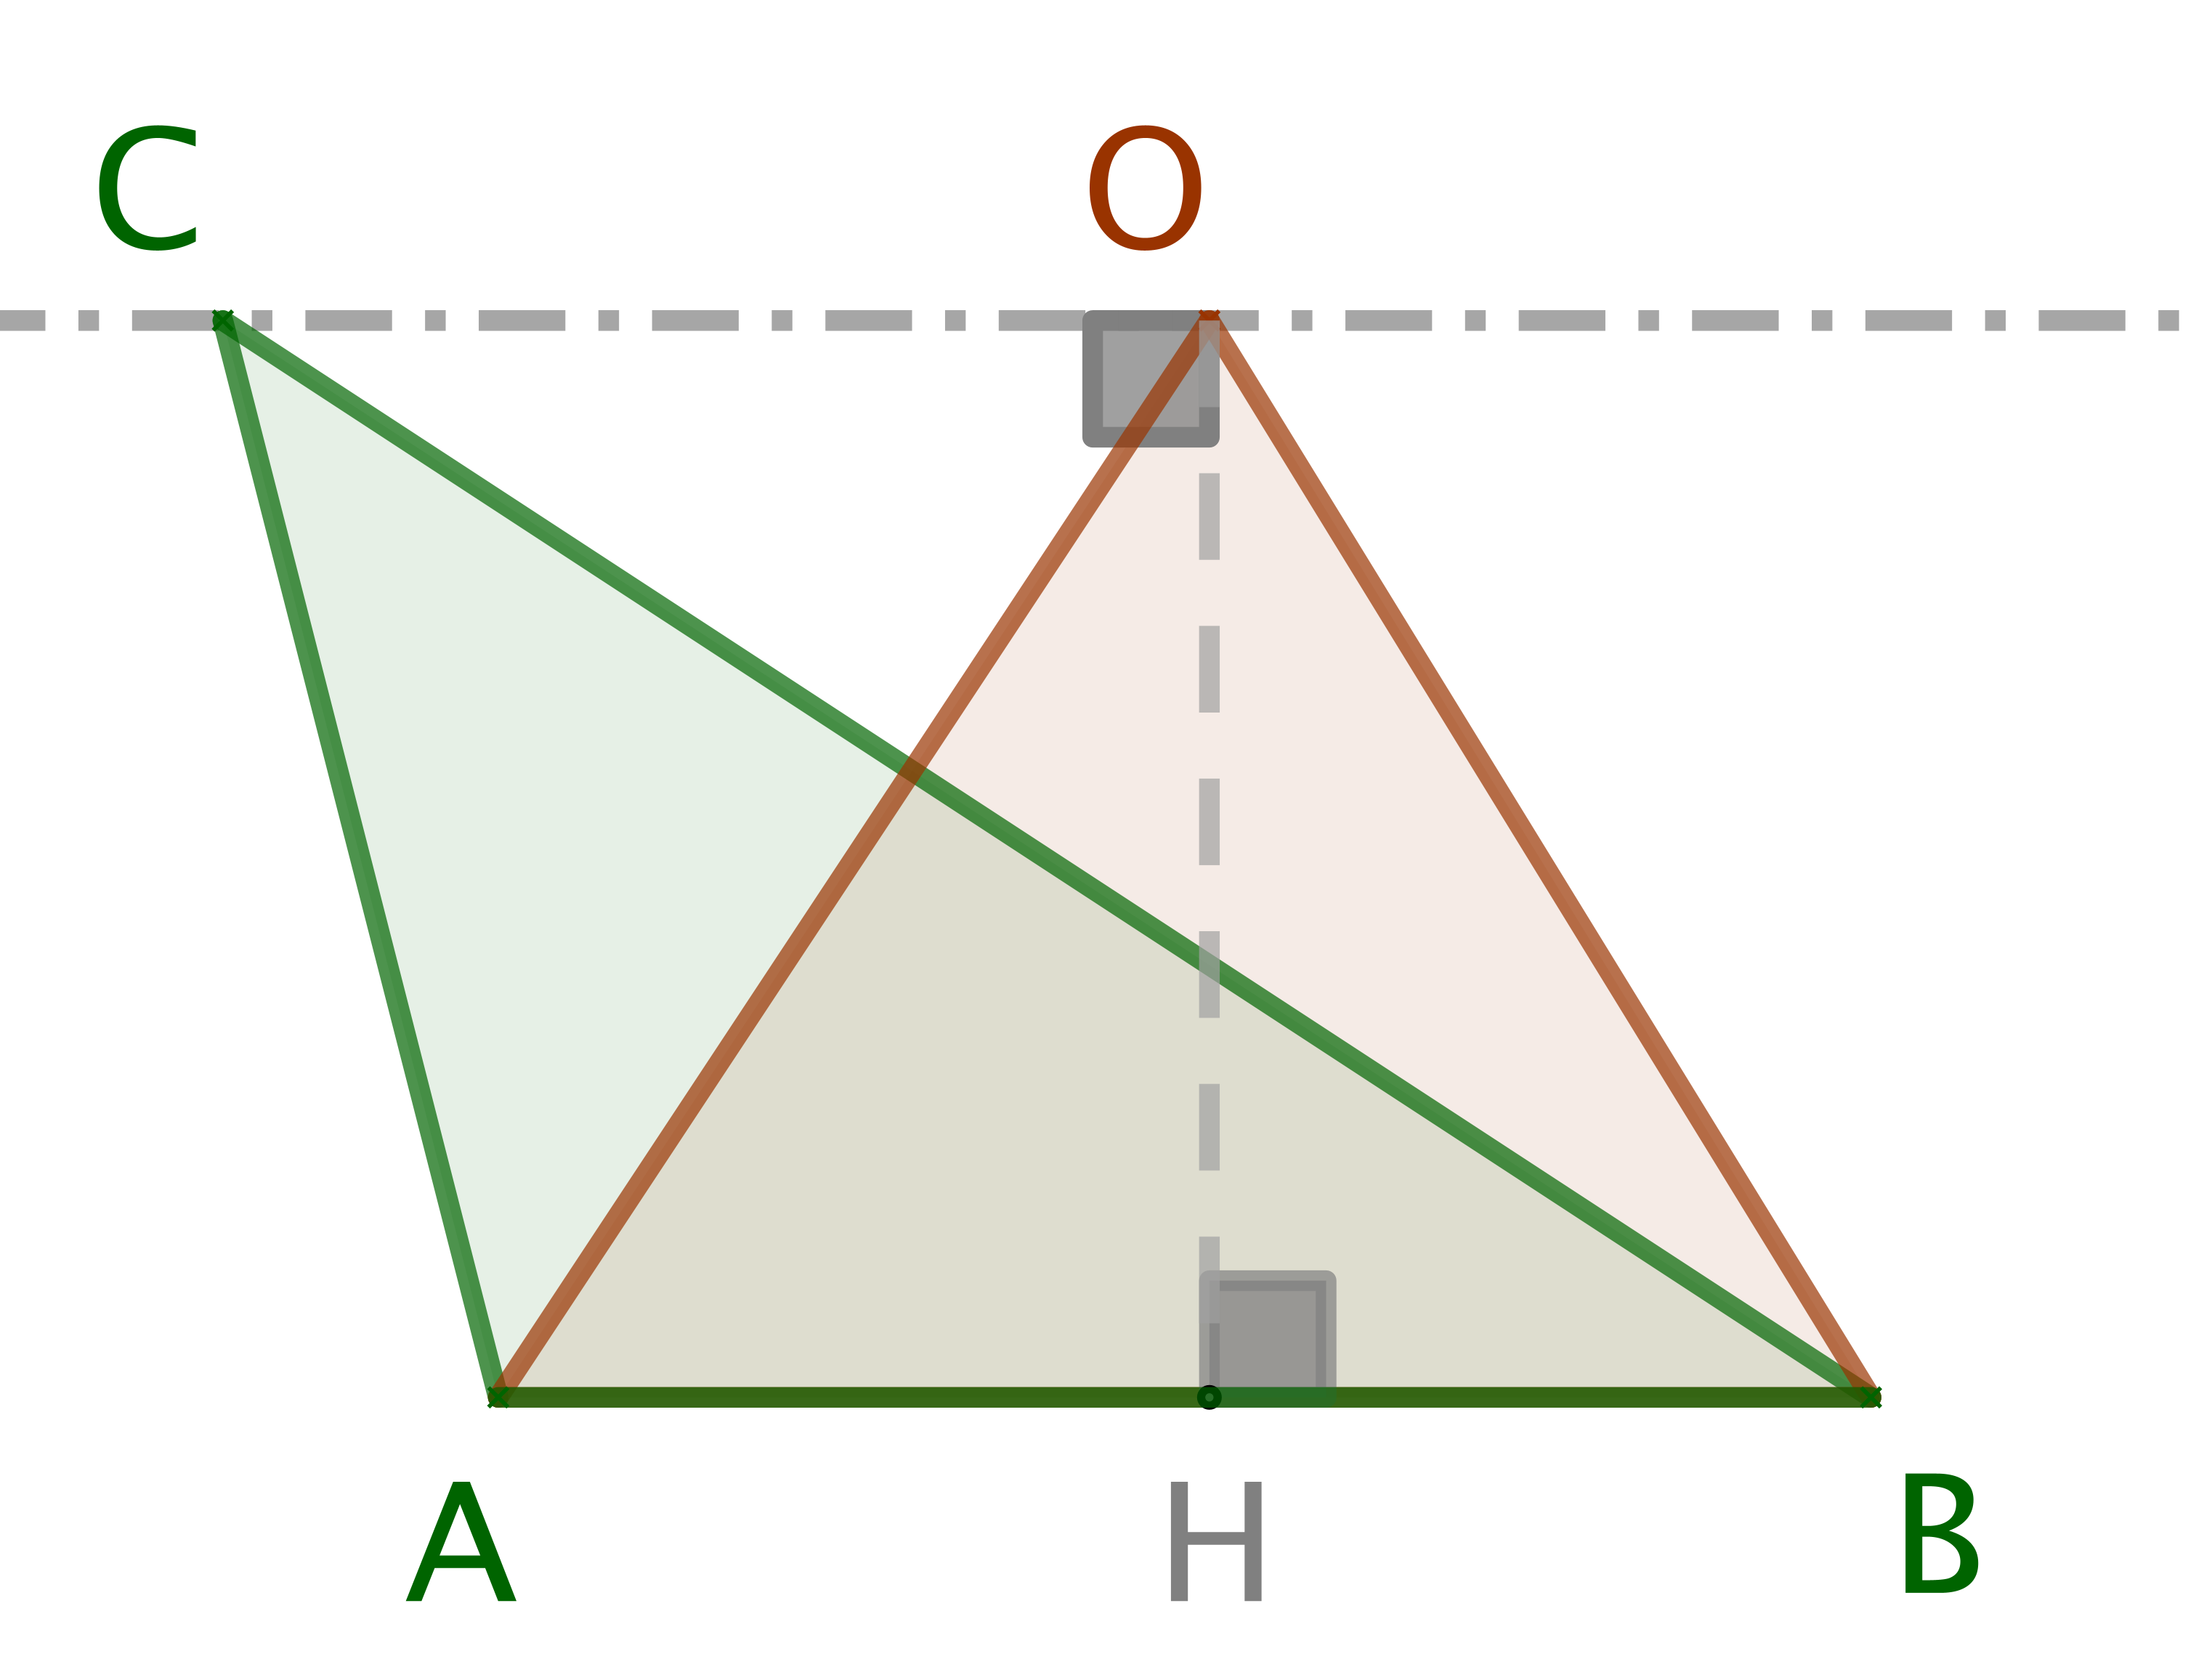
\includegraphics[scale=.4]{content/triangle-one-side-fixed/triangle.png}
	\end{center}

	
	Via une symétrie axiale, voir ci-dessous, il est aisé de noter que $\perim{ABC} \geq \perim{ABO}$, avec égalité uniquement si $ABC$ est isocèle en $C$.
	Plus précisément, en passant de $C$ à $O$, le périmètre diminue.
	
	\begin{center}
		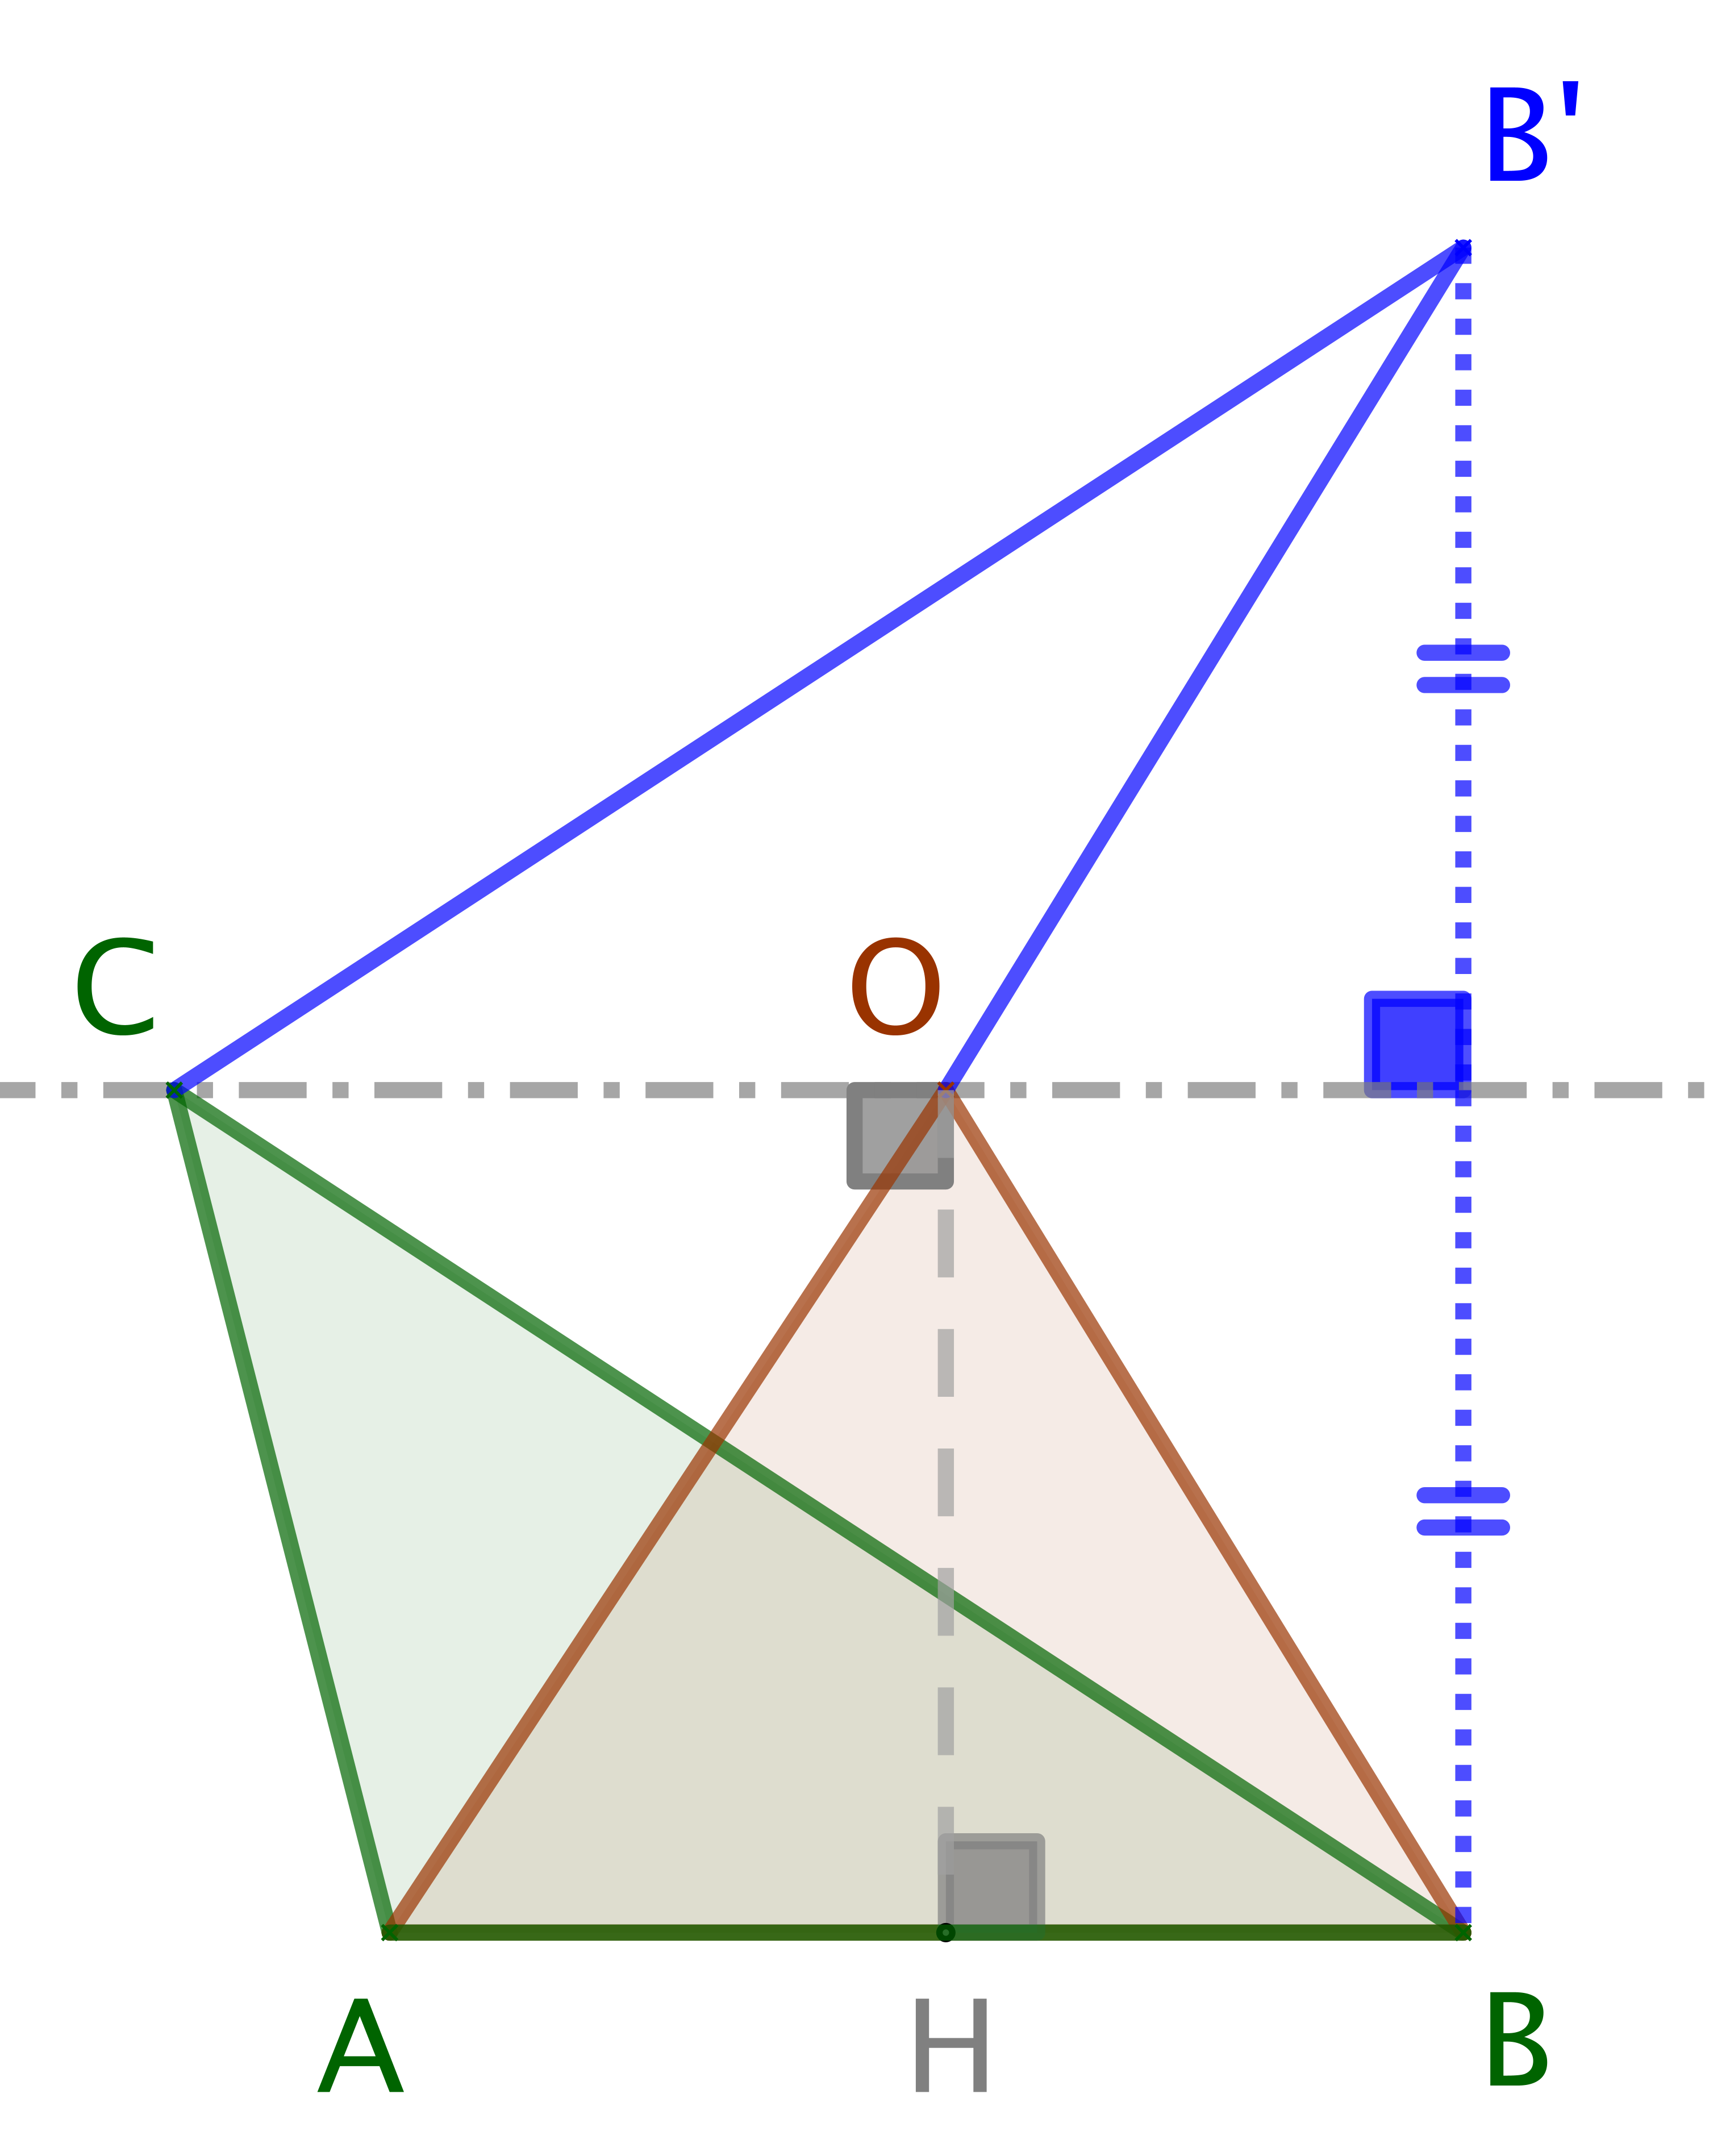
\includegraphics[scale=.4]{content/triangle-one-side-fixed/proof.png}
	\end{center}
	
	Une dilatation \focus{verticale} de rapport $r = \frac{\perim{ABC}}{\perim{ABO}} \geq 1$ donne un triangle isocèle $ABO^{\,\prime}$ tel que 
	$\perim{ABO^{\,\prime}} = p$
	et 
	$\area{ABO^{\,\prime}} \geq \area{ABC}$, avec égalité uniquement si $ABC$ est isocèle en $C$. 
	Contrat rempli!%
	\footnote{
		Dans la section \ref{constrained-extrema} est expliqué comment employer la méthode des extrema liés. 
		Les arguments fournis à cet endroit s'adaptent facilement au cas des triangles de base fixée.
	}
\end{proof}


% ----------------------- %


\begin{remark}
	La recherche parmi les triangles avec un côté fixé de celui ayant un périmètre minimal pour une aire fixée est le problème dual de l'isopérimétrie pour ces triangles.
\end{remark}

%
%
%% ------------- %
%
%
%\section{Les triangles sans contrainte}
%
%\begin{fact} \label{iso-tri}
	Considérons tous les triangles de périmètre fixé $p$. Parmi tous ces triangles, un seul est d'aire maximale, c'est le triangle équilatéral de côté $c = \dfrac13 p$.
\end{fact}


\begin{proof}	
	Nous allons donner une démonstration constructive via une application itérative du fait \ref{tri-one-side-fixed} qui va donner à la limite le triangle équilatéral d'aire maximale, et ceci avec une vitesse de convergence exponentielle.%
	\footnote{
		Ceci ne va nécessiter que l'emploi de propriétés simples de l'ensemble des réels.
	}
	Partons donc d'un triangle $ABC$ quelconque, mais de périmètre $p$, le fait \ref{tri-one-side-fixed} nous donne successivement les triangles $ACD$, $ADE$ et $AEF$ isocèles en $D$, $E$ et $F$ respectivement, ayant tous pour périmètre $p$, et ceci avec des aires de plus en plus grandes.  
	Le dessin suivant amène à conjecturer qu'en poursuivant le procédé pour avoir ensuite un triangle $AFG$ isocèle en $G$...\,, nous aboutirons \focus{à la limite} à un triangle équilatéral.

	\begin{center}
		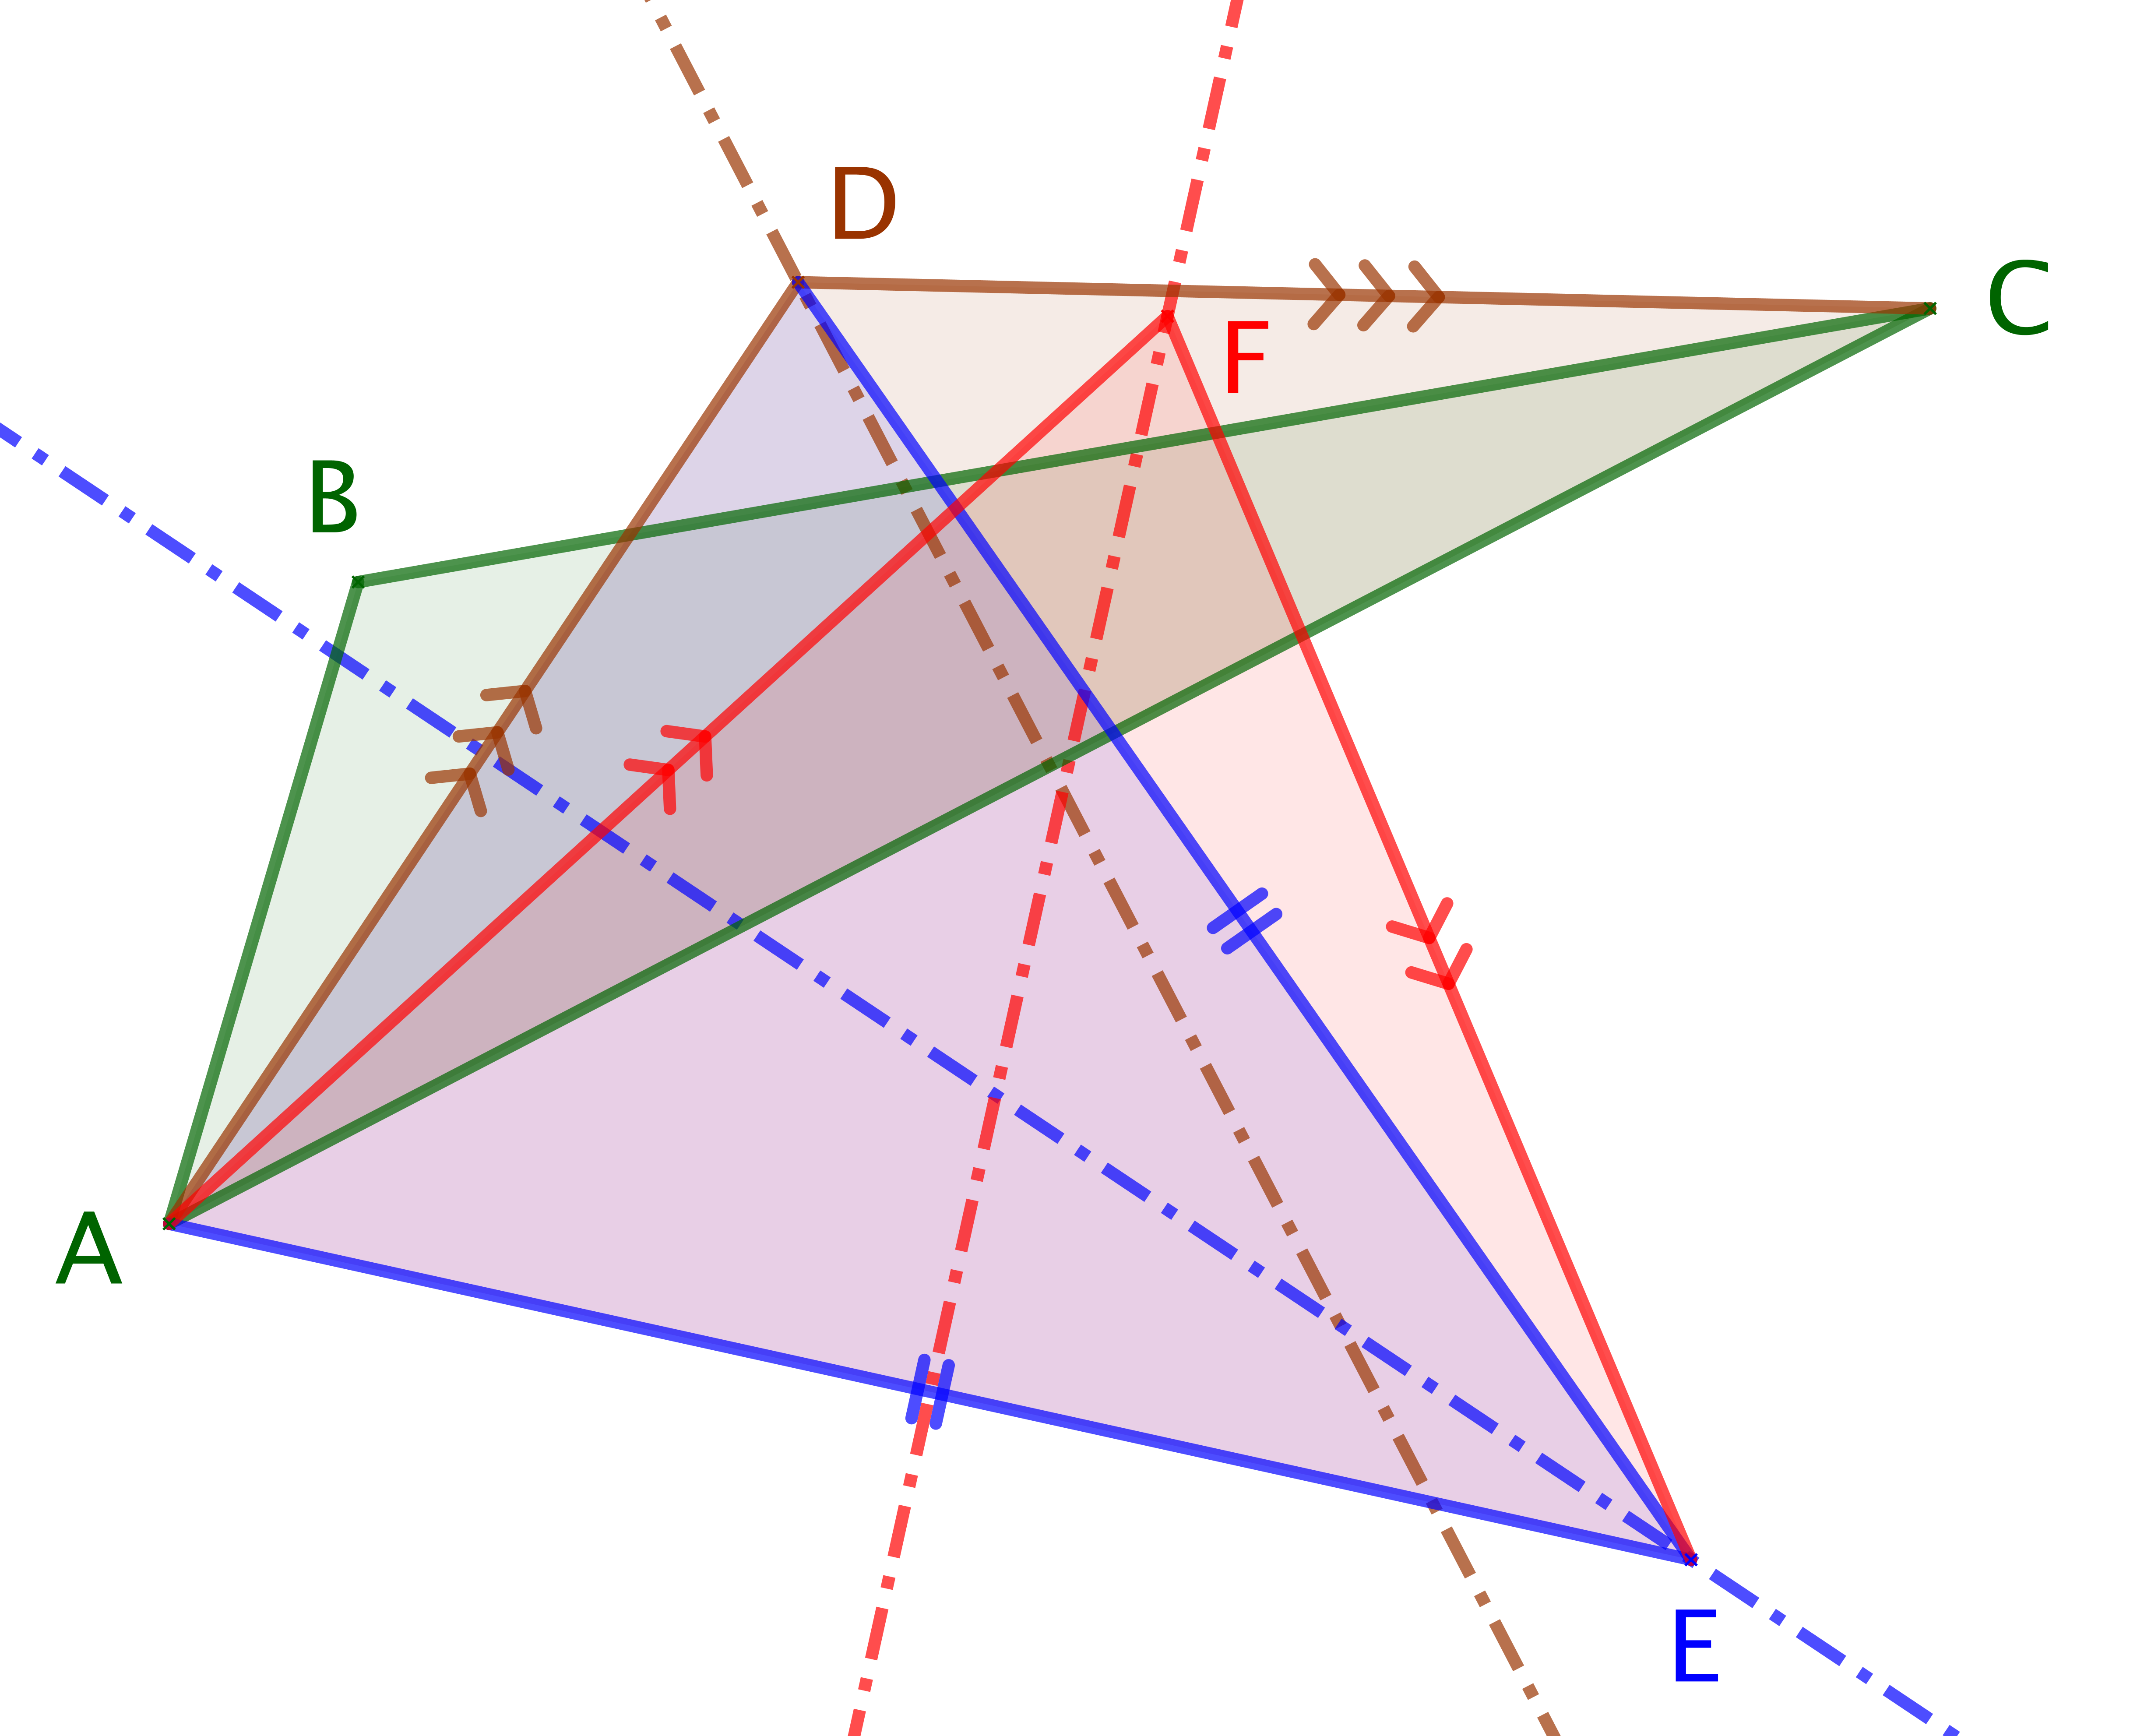
\includegraphics[scale=.4]{content/triangle-gene/proof.png}
	\end{center} 

	
	Le passage d'un triangle quelconque $ABC$ au triangle $ACD$ isocèle en $D$ nous amène à nous concentrer sur ce que donne notre procédé d'agrandissement d'aire à périmètre fixé pour des triangles isocèles. 
	Voici ce que nous pouvons affirmer en supposant $AC > AD$, comme dans notre exemple (nous allons voir que cette hypothèse est sans conséquence).
	%
	\begin{enumerate}
		\item Comme $AC + 2 AD = p$ et $AC > AD$, nous avons $AC > \frac13 p > AD$.
		À l'étape suivante, comme $AD + 2 AE = p$, nous obtenons $AD < \frac13 p < AE$.


		\item Pour $AEF$ isocèle en $F$, comme $AE + 2AF = p$, nous arrivons à  $AE > \frac13 p > AF$.
		
		
		\item \label{tri-equi-conv}
		Tentons de quantifier les écarts à la mesure pivot $p^{\,\prime} = \frac13 p$. 
		%
		\begin{itemize}
			\item Dans $ACD$, posant $AD = p^{\,\prime} - \epsilon_1$, nous avons $AC = p^{\,\prime} + 2 \epsilon_1$.

			\item Dans $ADE$, posant $AE = p^{\,\prime} + \epsilon_2$, nous avons $AD = p^{\,\prime} - 2 \epsilon_2$.

			\item Dans $AEF$, posant $AF = p^{\,\prime} - \epsilon_3$, nous avons $AE = p^{\,\prime} + 2 \epsilon_3$.

			\item Dans $AFG$, posant $AG = p^{\,\prime} + \epsilon_4$, nous avons $AF = p^{\,\prime} - 2 \epsilon_4$.

			\item Donc
			$\epsilon_2 = \frac12 \epsilon_1$,
			$\epsilon_3 = \frac12 \epsilon_2$
			et
			$\epsilon_4 = \frac12 \epsilon_3$.
		\end{itemize}
	\end{enumerate}


	\smallskip
	
	Voici les enseignements de ce qui précède en partant d'un triangle $ABC$ non équilatéral.
	%
	\begin{itemize}
		\item Si $AC = \frac13p$, dès la 1\iere\ itération, nous avons un triangle équilatéral d'aire plus grande.
		
		
		\item Si $AC \neq \frac13p$, notre procédé n'arrivera jamais en un nombre fini d'étapes à un triangle équilatéral.
		Dans ce cas, le point \ref{tri-equi-conv} ci-dessus nous donne une convergence exponentielle des longueurs des côtés vers $p^{\,\prime} = \frac13 p$, tout en ayant des aires des plus en plus grandes.
	\end{itemize}
	
	Dans tous les cas, l'aire d'un triangle non équilatéral de périmètre $p$ est strictement majorée par celle du triangle équilatéral de périmètre $p$. Et tout ceci a été obtenu via de la géométrie et de l'analyse élémentaires!
\end{proof}

%
%
%% ------------- %
%
%
%\section{Les quadrilatères}
%
%\begin{fact}
	Considérons tous les quadrilatères de périmètre fixé $p$. Parmi tous ces quadrilatères, celui d'aire maximale est le carré de côté $c = \num{.25} p$.
\end{fact}


\begin{proof}
	La figure suivante montre que pour tout quadrilatère $ABCD$ non convexe en $B$, et de périmètre $p$, il existe un quadrilatère convexe $AB^{\,\prime}CD$ de périmètre $p$, et tel que $\area{AB^{\,\prime}CD} \geq \area{ABCD}$.
	Notre recherche doit donc continuer dans l'ensemble des quadrilatères convexes de périmètre $p$.

	\begin{center}
		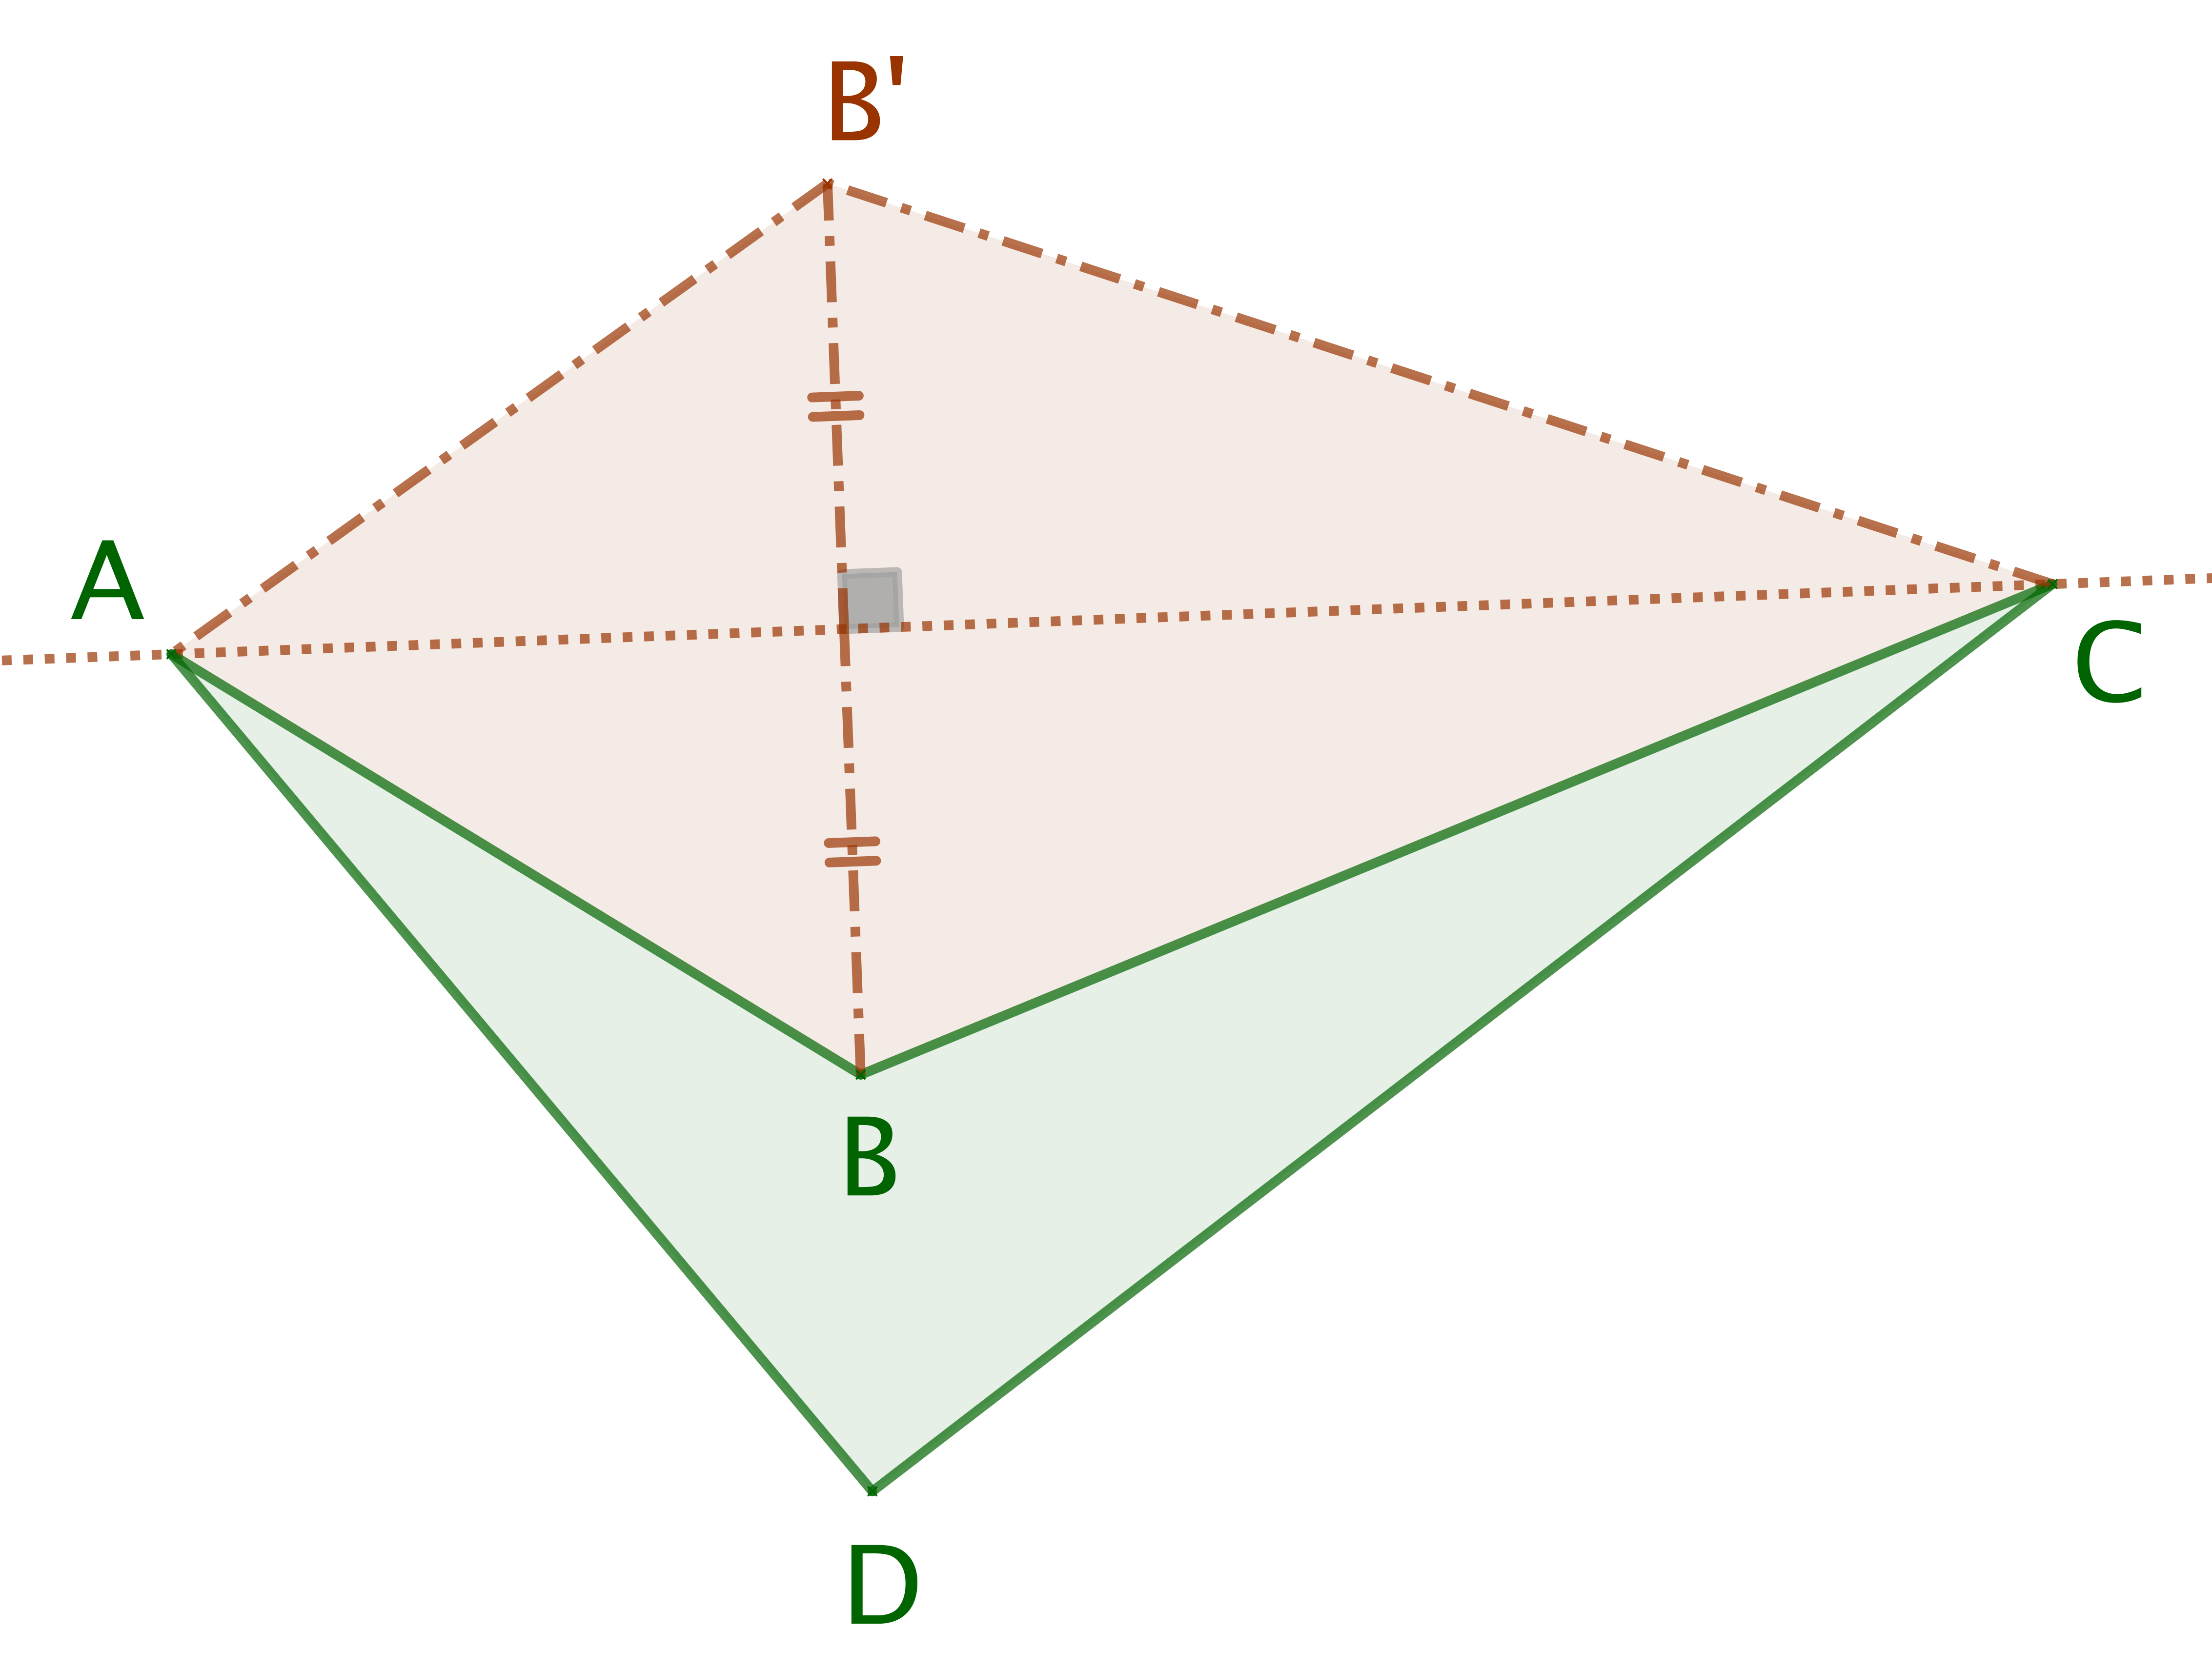
\includegraphics[scale=.4]{content/quadrilateral/quadrilateral-non-convex.png}
	\end{center}
	
	
	Comme dans la preuve du fait \ref{iso-tri-one-side-fixed}, à partir d'un quadrilatère convexe $ABCD$ de périmètre $p$, nous obtenons un quadrilatère convexe $AB^{\,\prime}CD$ de périmètre $p$,%
	\footnote{
		Noter que
		$\perim{AB^{\,\prime}CD} = \perim{AB^{\,\prime}C} + \perim{ACD} - 2 AC$.
	}
	et tel que $AB^{\,\prime} = B^{\,\prime}C$ et $\area{AB^{\,\prime}CD} \geq \area{ABCD}$ comme le montre la figure ci-après. 

	\begin{center}
		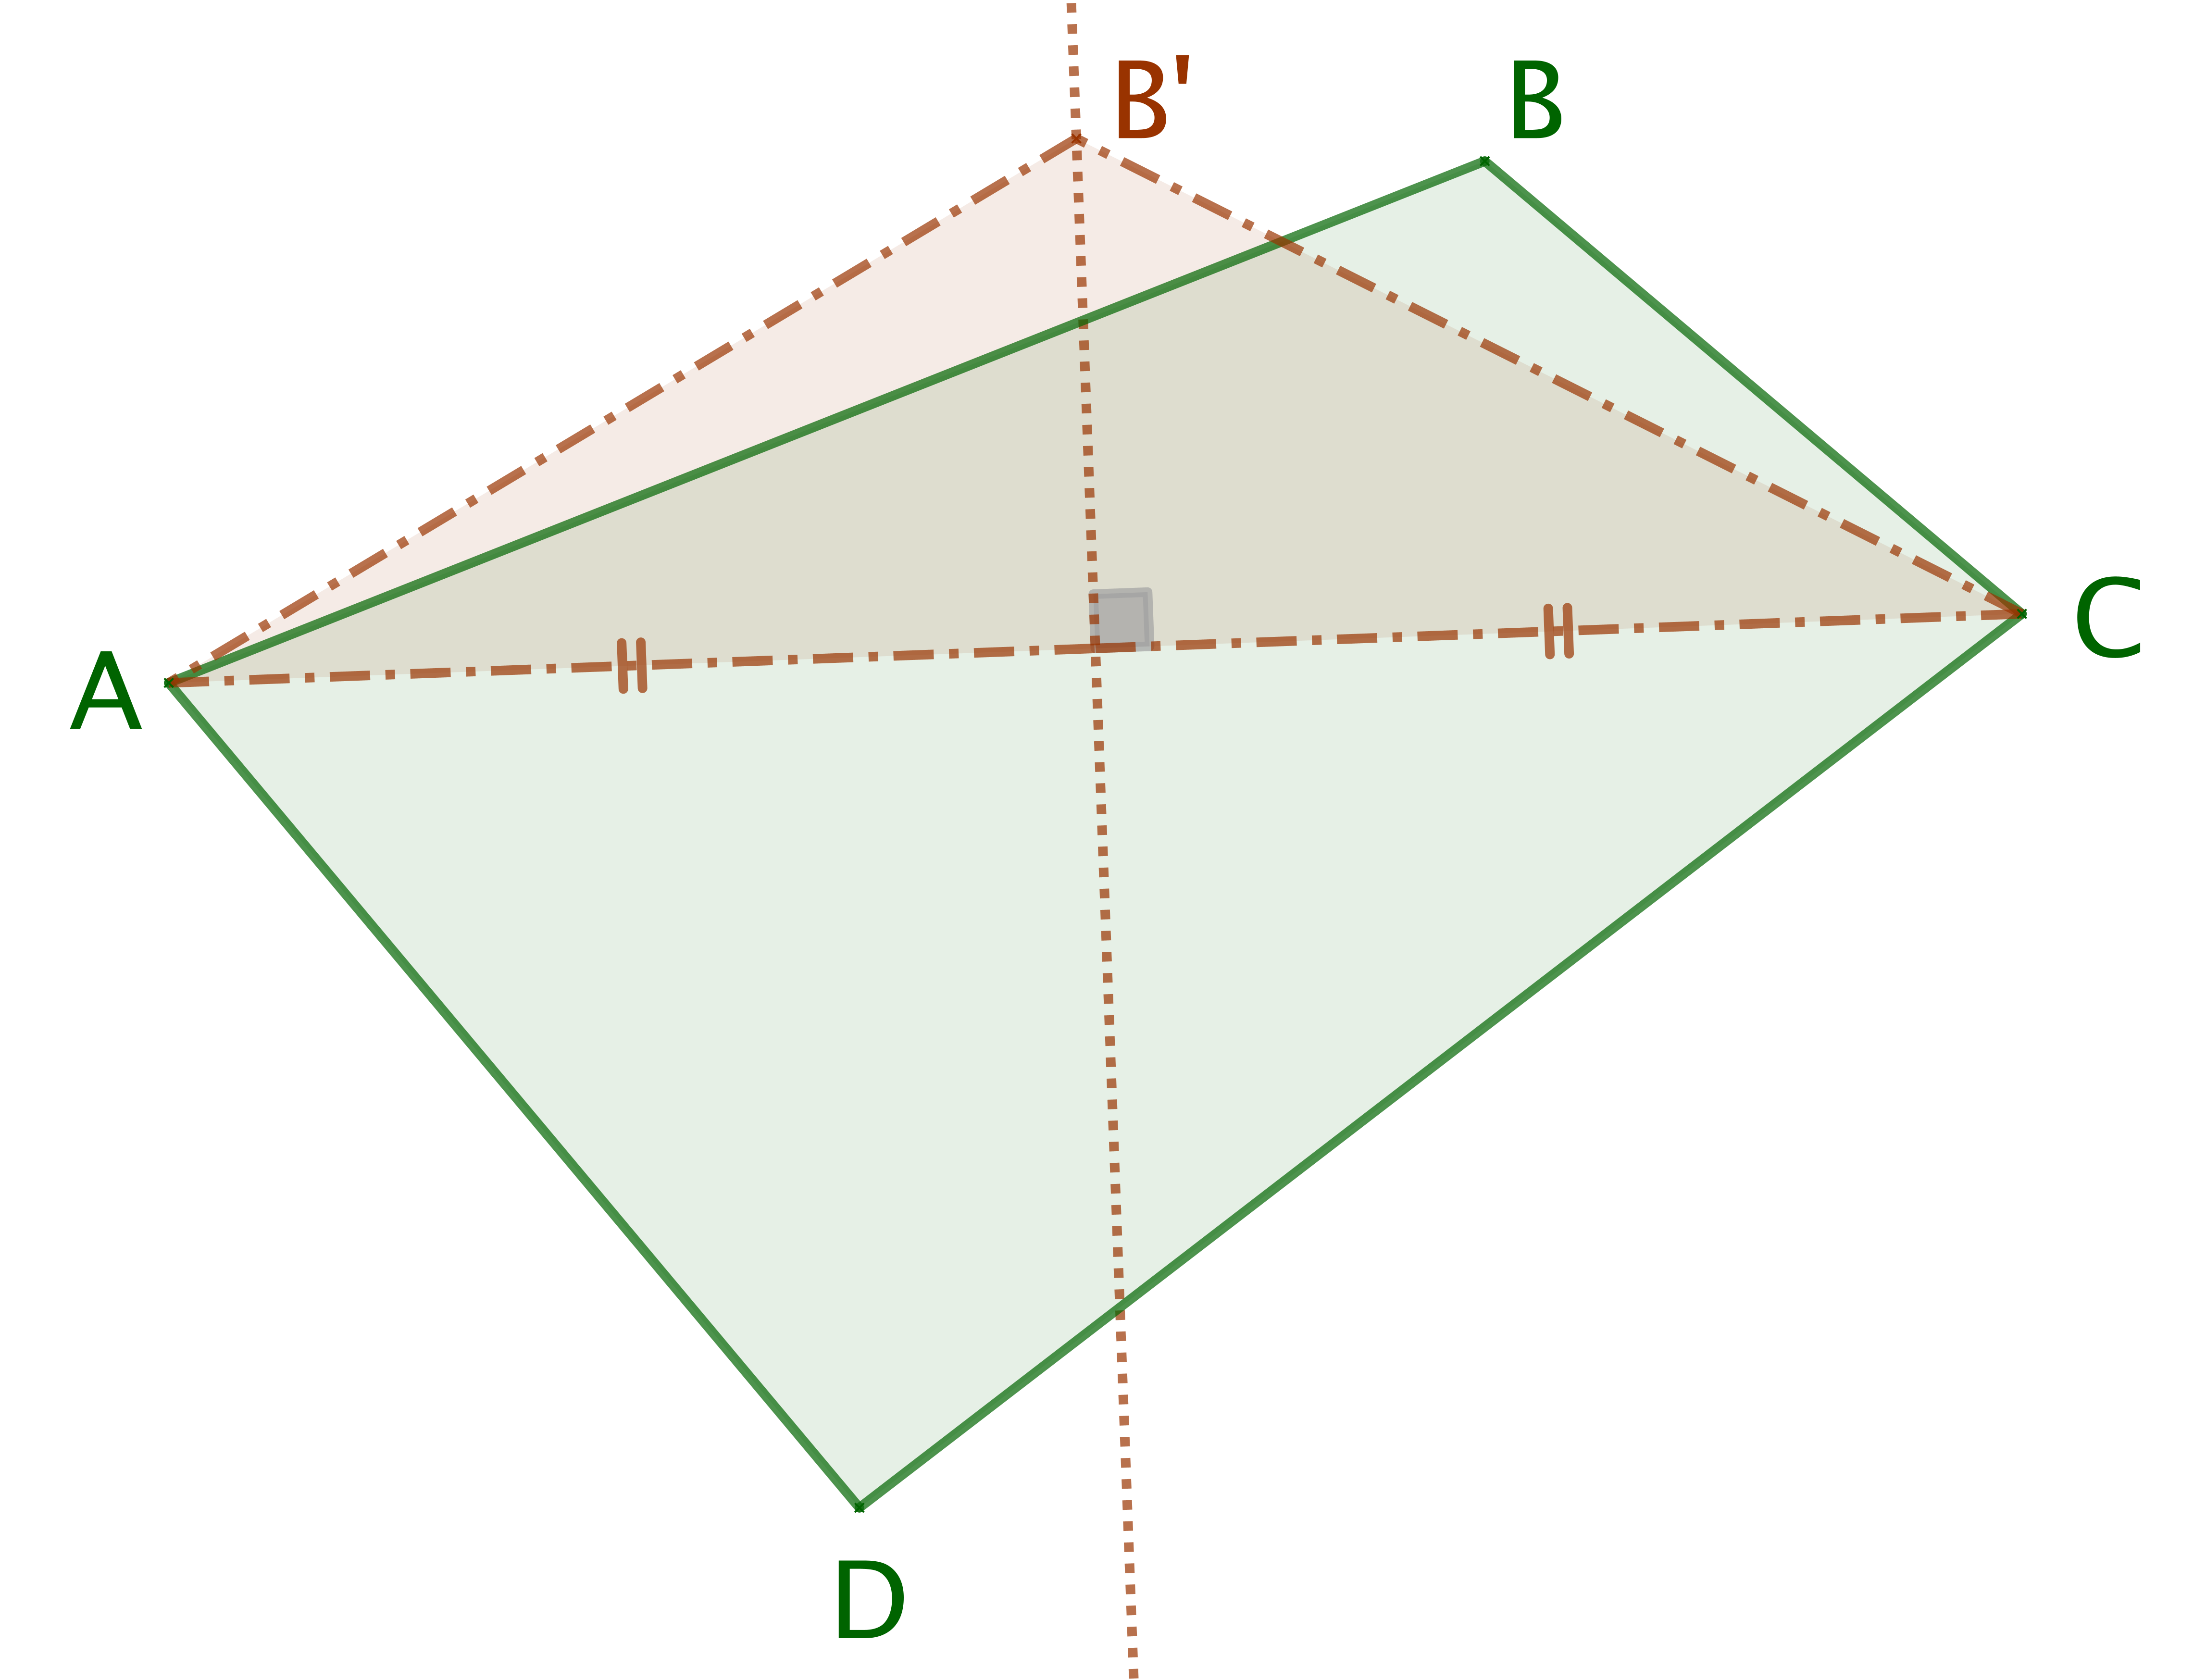
\includegraphics[scale=.4]{content/quadrilateral/quadrilateral-convex-gene.png}
	\end{center}
	
	
	La méthode précédente appliquée au sommet $D$ donne un cerf-volant $ABCD$ de périmètre $p$, et tel que $AB = BC$ et $AD = DC$, voir ci-dessous. 
	Cette même méthode avec les sommets $A$ et $C$ fournit un losange $A^{\,\prime}BC^{\,\prime}D$ de périmètre $p$, et tel que $\area{A^{\,\prime}BC^{\,\prime}D} \geq \area{ABCD}$.
	%
	En effet, nous avons
	$p = 2(AB + AD)$
	et
	$\perim{A^{\,\prime}BD} = \perim{ABD}$,
	donc
	$A^{\,\prime}B = A^{\,\prime}D = \num{.25} p$,
	et de même, nous obtenons
	$C^{\,\prime}B = C^{\,\prime}D = \num{.25} p$.

	\begin{center}
		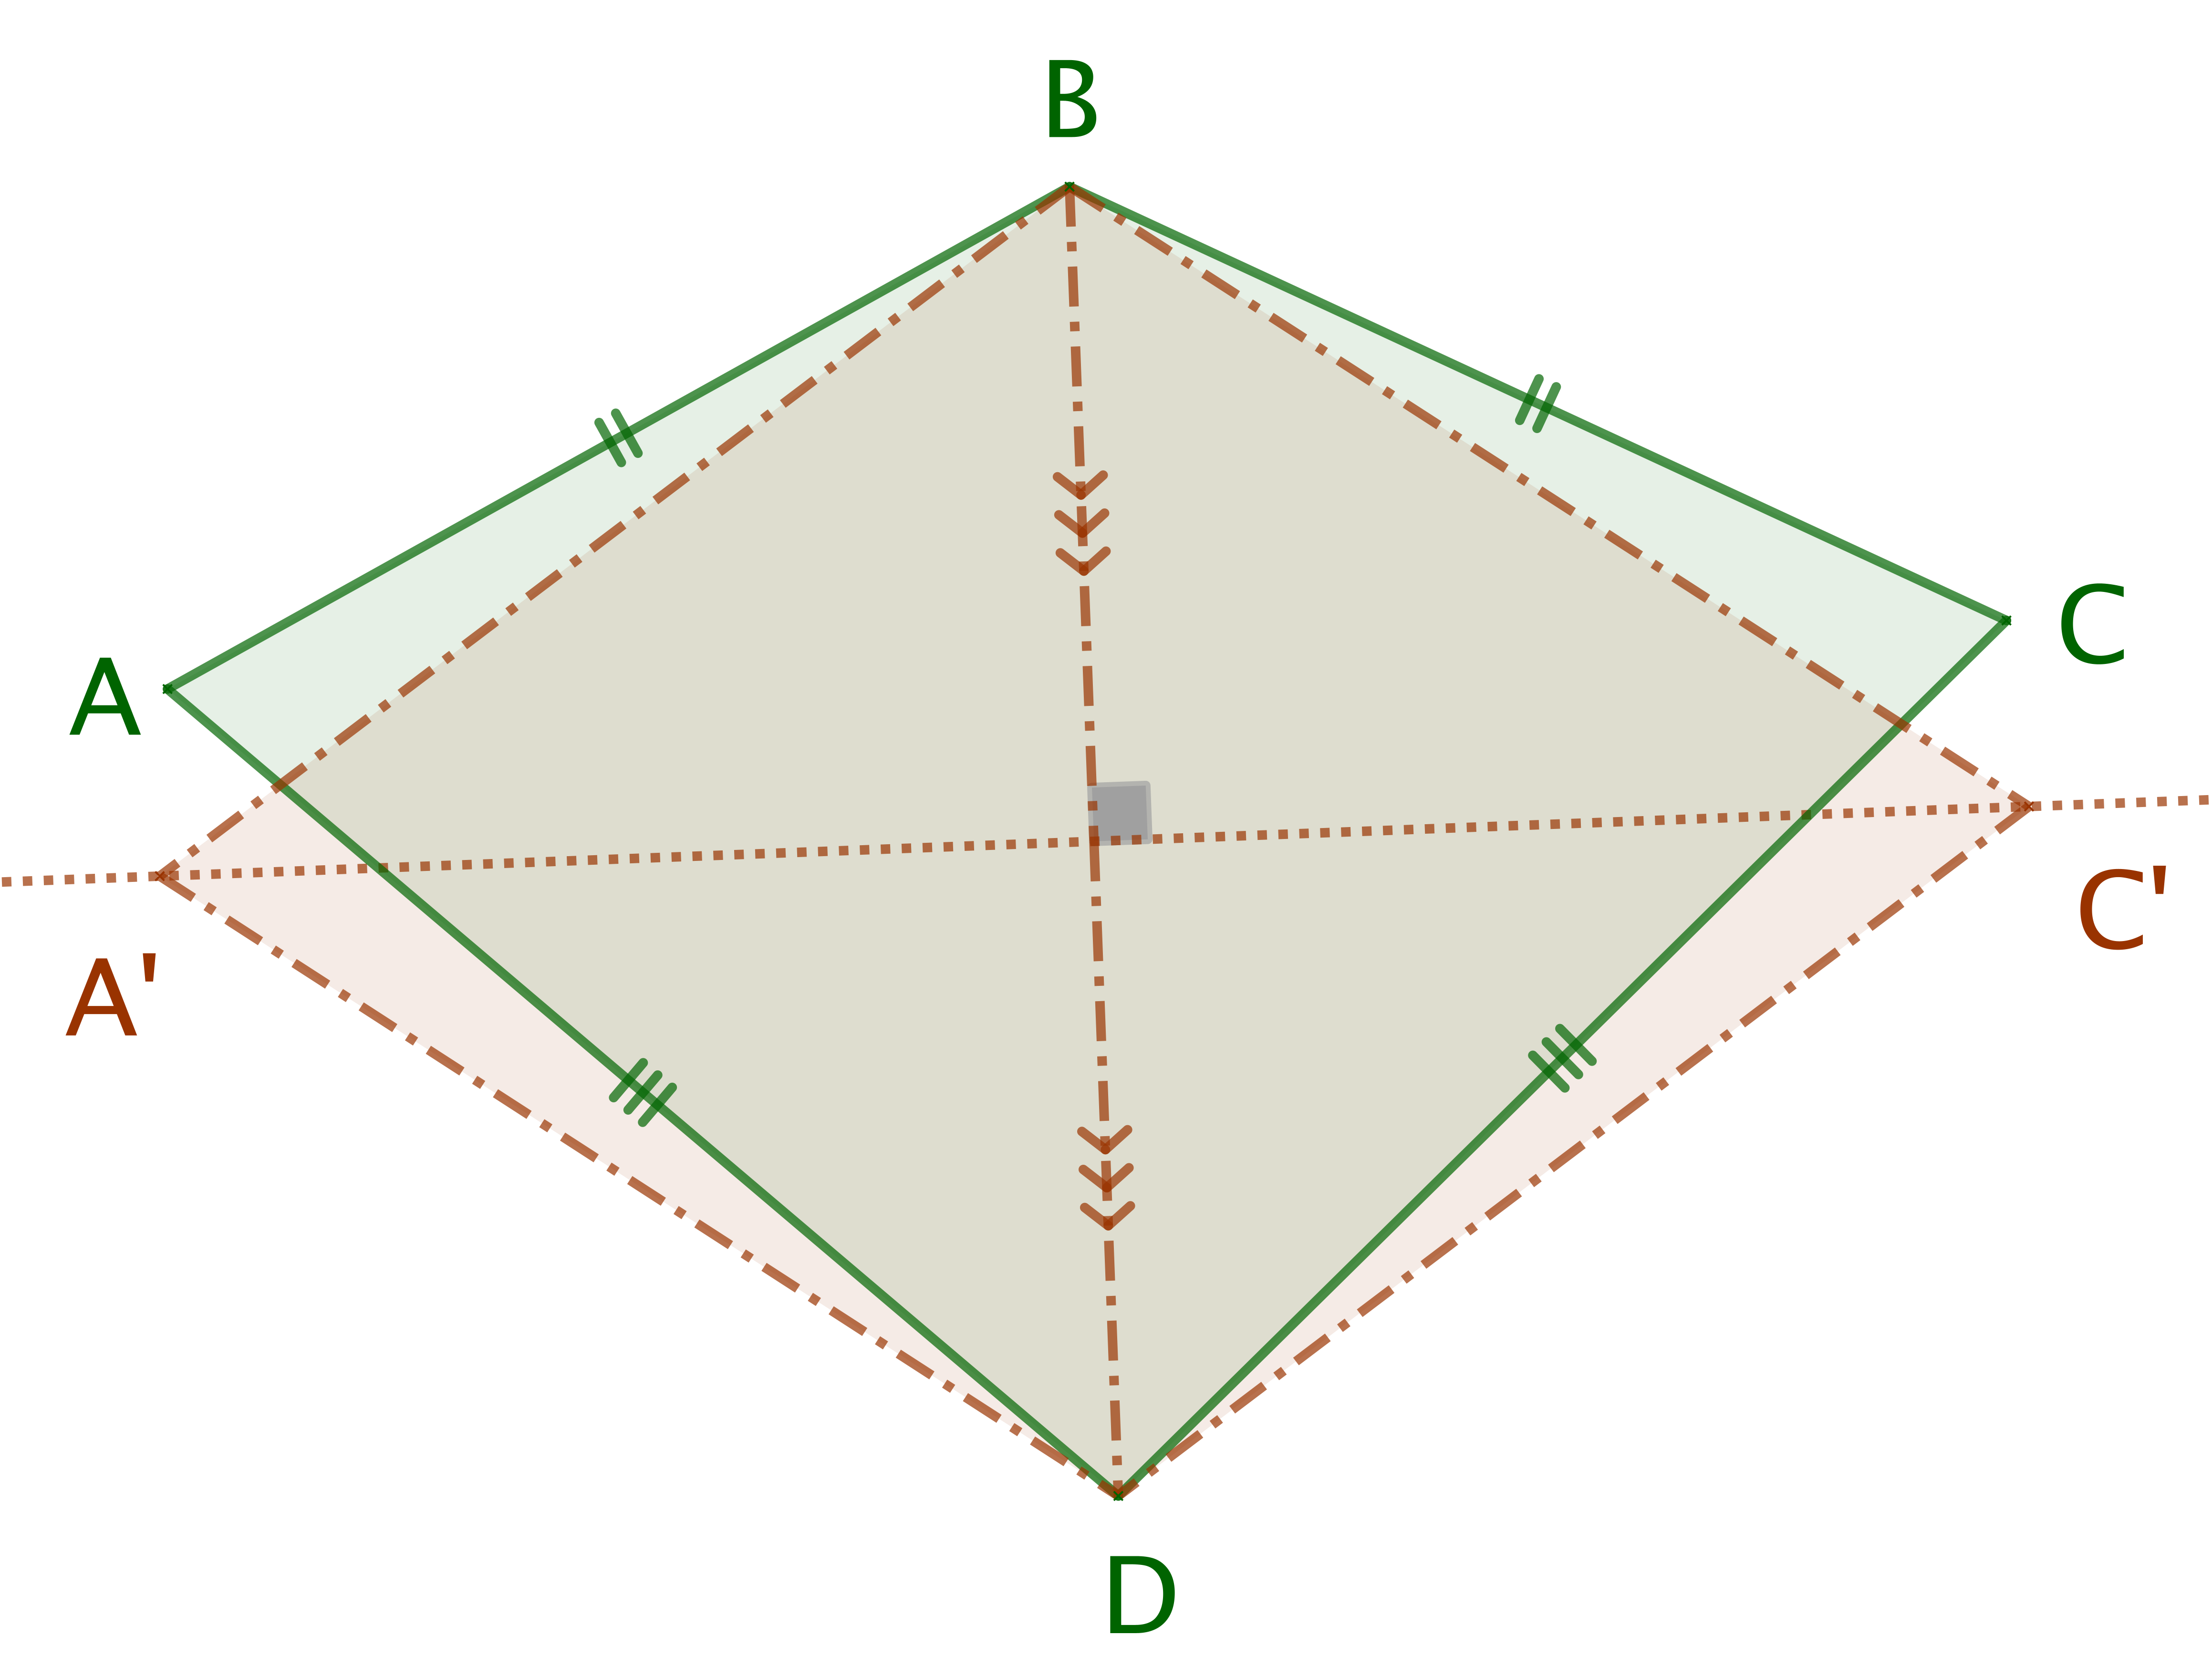
\includegraphics[scale=.4]{content/quadrilateral/quadrilateral-convex-isopaire.png}
	\end{center}
	
	
	Pour conclure, il suffit d'appliquer le fait \ref{iso-para}, puisque tout losange est un parallélogramme. Que la géométrie est belle!
\end{proof}


%
%
%% ------------- %


\section{Les polygones}

La technique ne change pas: nous allons restreindre la recherche à des polygones de plus en plus particuliers. Cette dernière section nous poussera à un peu plus de technicité.


% ----------------------- %


\begin{defi}
	Un \og \emph{$n$-gone} \fg\ désigne un polygone à $n$ côtés avec $n \geq 3$.
\end{defi}


\begin{defi}
	Un \og \emph{$n$-isogone} \fg\ désigne un $n$-gone dont tous les côtés sont de mesure égale.
\end{defi}


% ----------------------- %


\begin{fact}\label{conv-poly}
	Si un $n$-gone $\setproba{P}$, de périmètre fixé $p$, n'est pas convexe, alors on peut construire à partir de $\setproba{P}$ un $n$-gone convexe $\setproba{P}^{\,\prime}$ tel que $\perim{\setproba{P}^{\,\prime}} = p$ et $\area{\setproba{P}^{\,\prime}} > \area{\setproba{P}}$.
\end{fact}


\begin{proof}
	Ici, il ne faut pas être expéditif en indiquant que la preuve du fait \ref{quadri} se généralise sans aucun souci.
	En effet, avec $n > 4$, nous pouvons avoir plusieurs points de non-convexité, et les éliminer comme nous l'avons fait pour le quadrilatère n'est pas immédiat:
	dans la figure suivante, l'élimination des deux points de non convexité $G$ et $E$ de l'heptagone $ABCDEFG$ nous amène à un nouvel heptagone $ABCDE^{\,\prime}FG^{\,\prime}$ ayant lui aussi deux points de non-convexité $F$ et $D$!
	Donc, rien n'empêche, a priori, d'avoir une suite de constructions n'aboutissant jamais à un heptagone convexe%
	\footnote{
		L'auteur est convaincu que le procédé aboutira en un nombre fini d'étapes à un polygone convexe, mais il ne l'a pas démontré pour le moment.
	}
	de même périmètre que celui de $ABCDEFG$, et d'aire strictement supérieure à celle de $ABCDEFG$.

	\begin{center}
		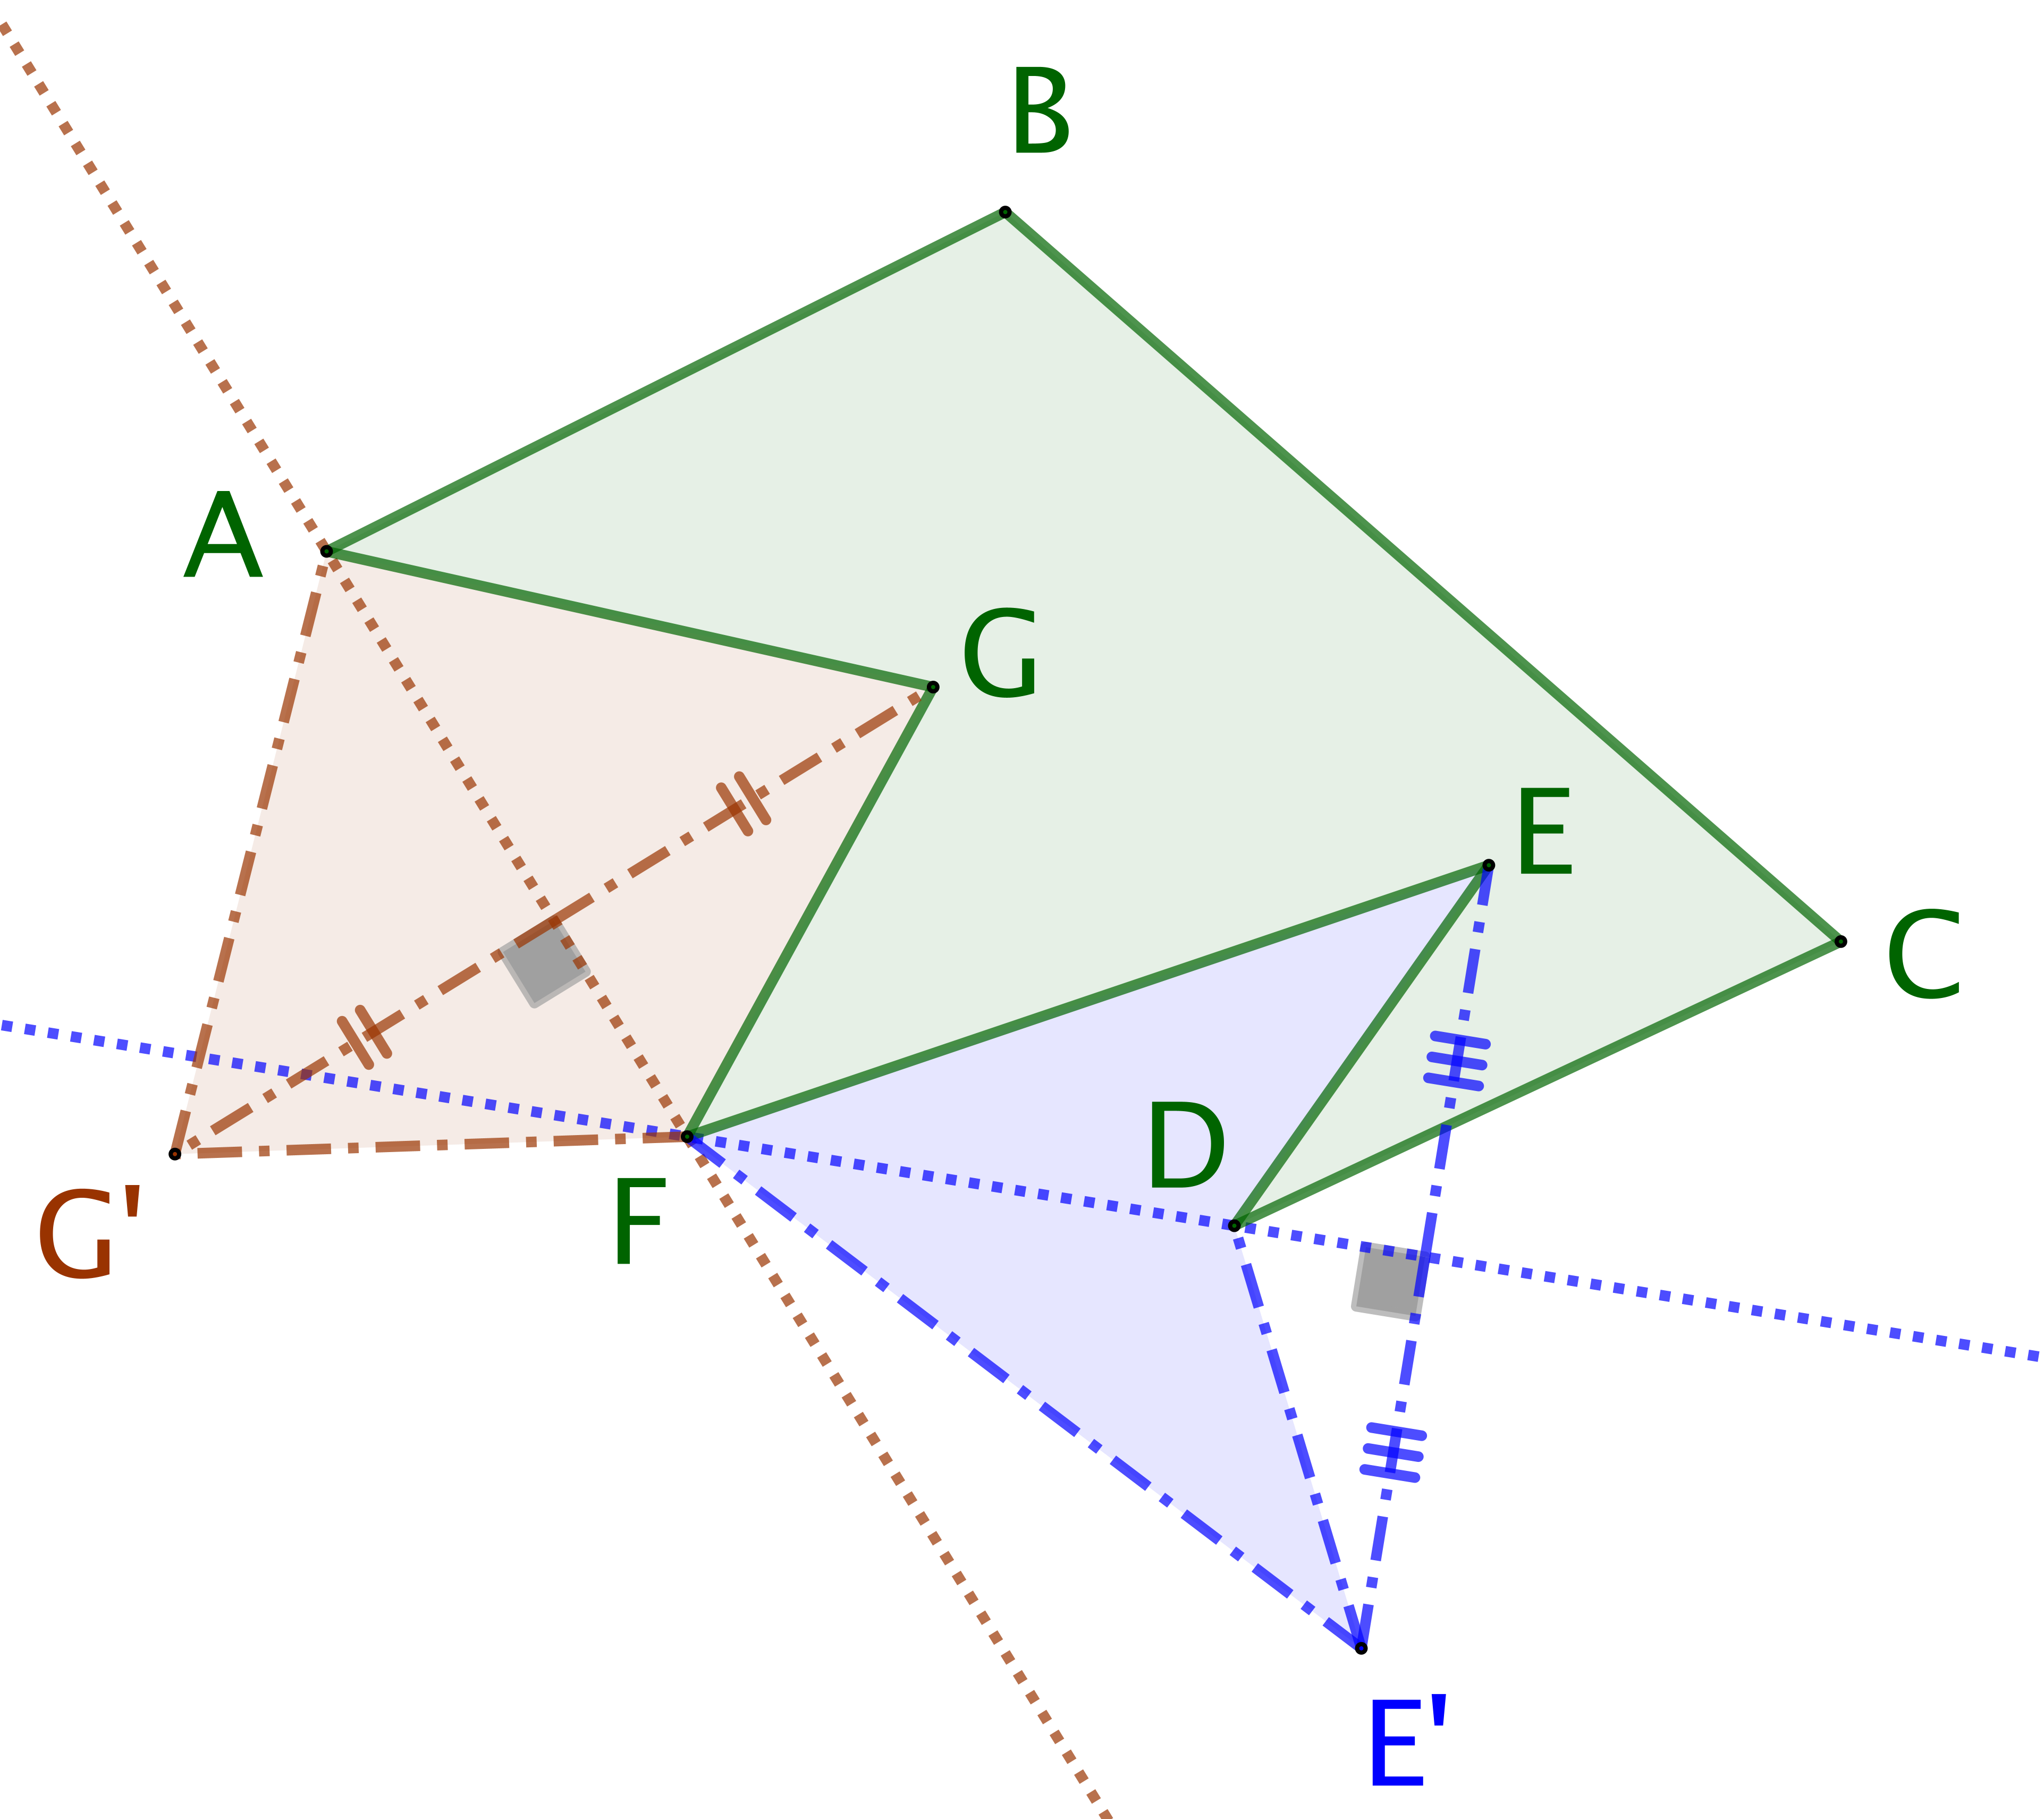
\includegraphics[scale=.4]{content/polygon/polygon-non-convex-trap.png}
	\end{center}
	

	Pire, on peut perdre des côtés lors de la construction comme dans l'exemple suivant où $C$, $D$ et $E^{\,\prime}$ sont alignés.

	\begin{center}
		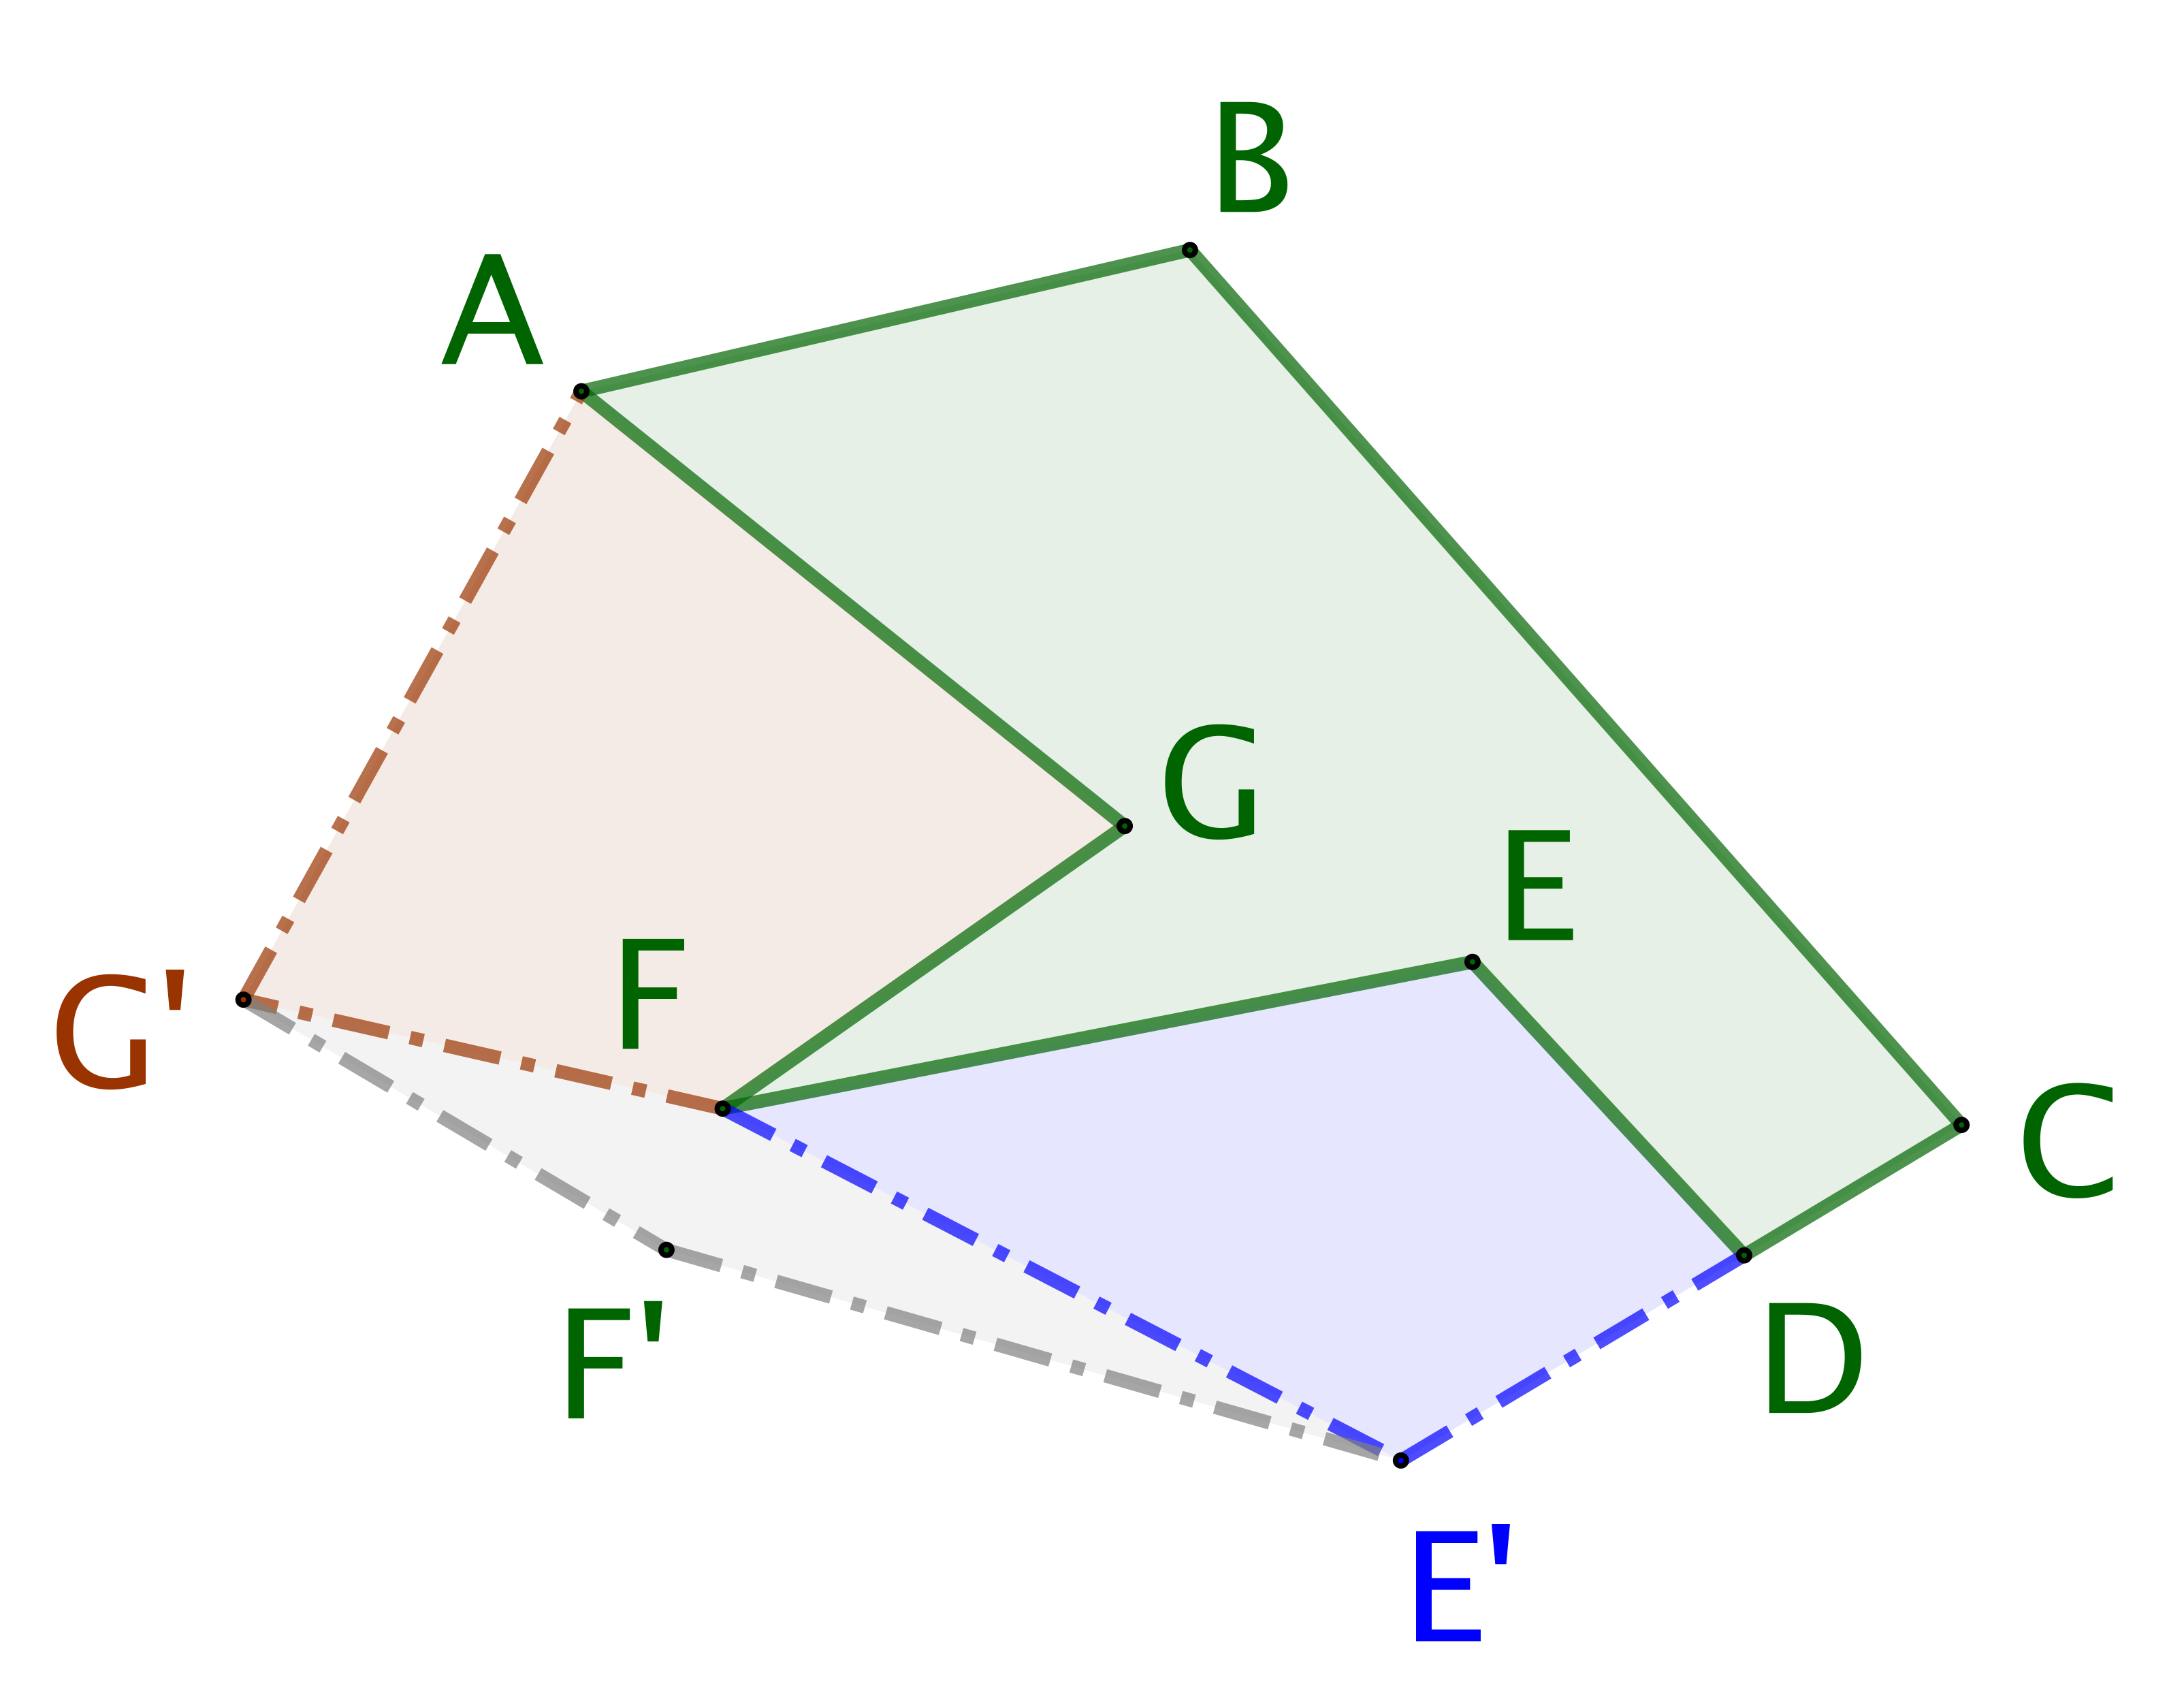
\includegraphics[scale=.4]{content/polygon/polygon-non-convex-bad.png}
	\end{center}


	Laissons de côté cette construction pour nous concentrer sur la classique enveloppe convexe%
	\footnote{
		C'est le plus petit polygone convexe \og \emph{contenant} \fg\ le $n$-gone considéré, où \og \emph{petit} \fg\ est relatif à l'inclusion.
	}
	du $n$-gone de départ dont les dimensions sont maitrisées par les sommets du $n$-gone.
	Par exemple, l'ennéagone $ABCDEFGHI$ non convexe ci-dessous admet le pentagone $ABDEG$ pour enveloppe convexe: le périmètre diminue et l'aire augmente, ce qui est utile, mais malheureusement le nombre de côtés change.
	
	\begin{center}
		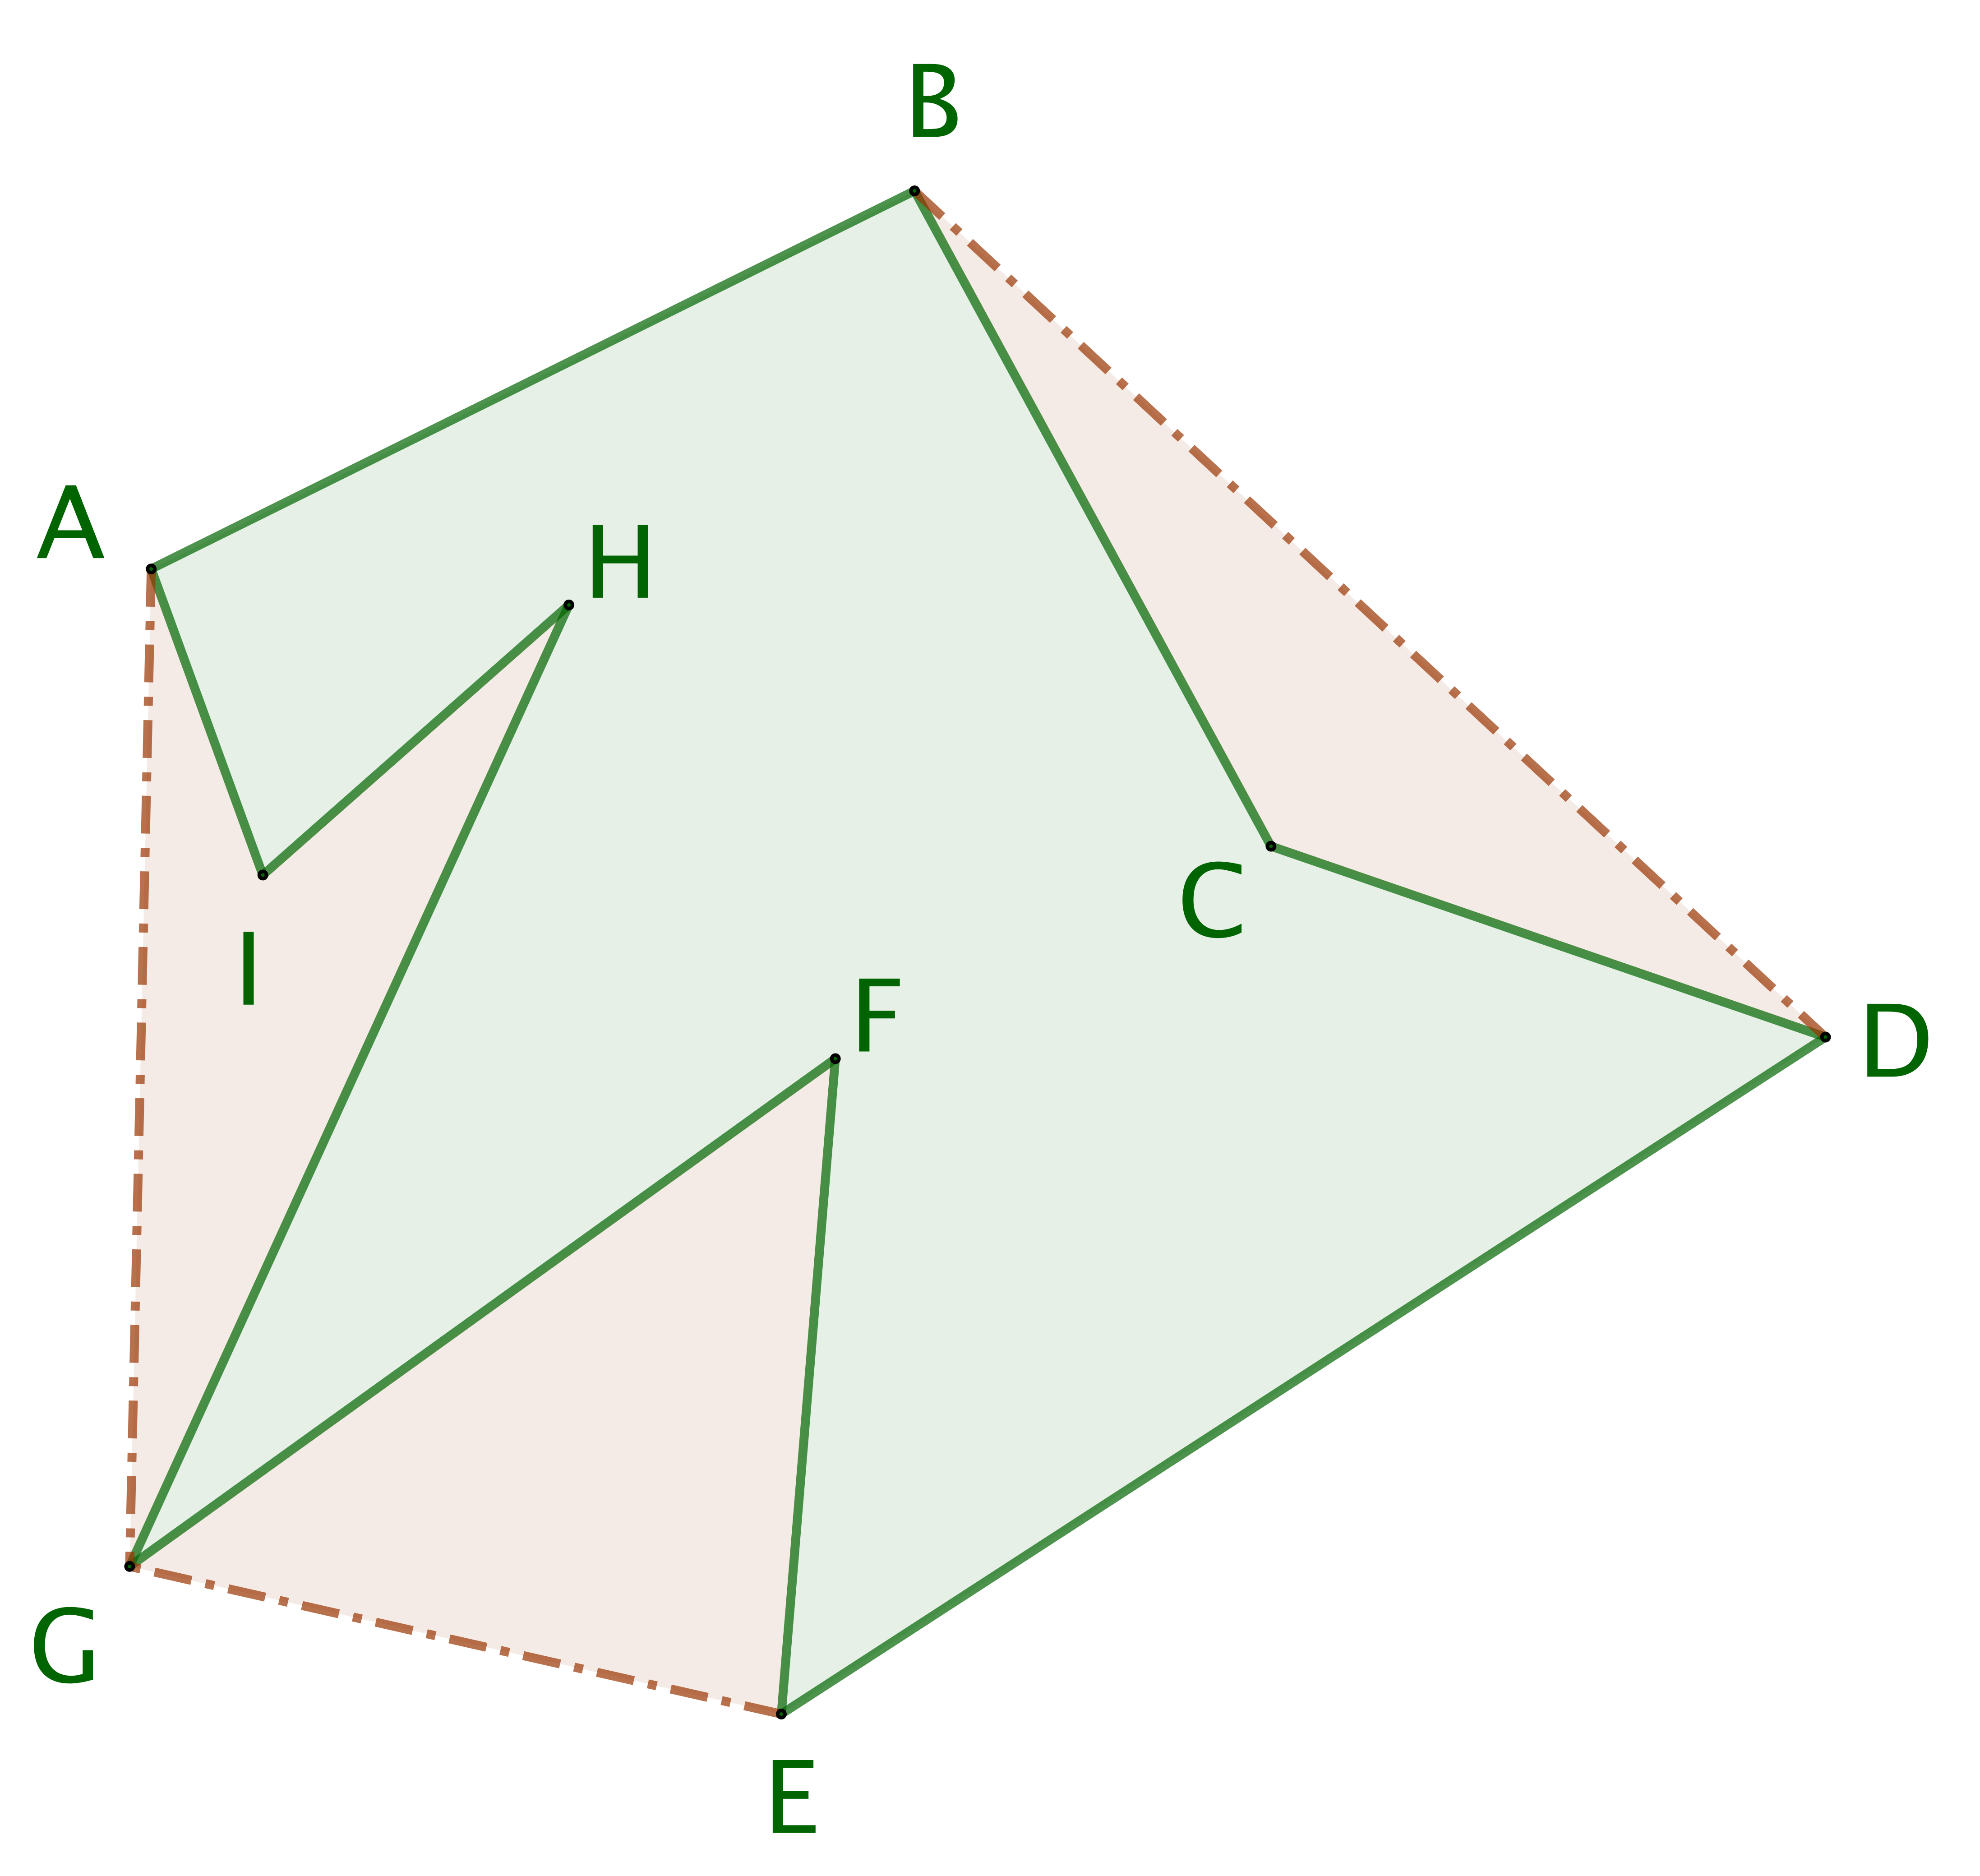
\includegraphics[scale=.4]{content/polygon/polygon-convex-hull.png}
	\end{center}

	Une idée simple, que nous allons formaliser rigoureusement juste après, consiste à ajouter les sommets manquants suffisamment prêts des côtés de l'enveloppe convexe afin de ne pas trop augmenter le périmètre afin qu'il ne dépasse pas celui du $n$-gone non convexe initial. Le dessin suivant illustre cette idée.	
	
	\begin{center}
		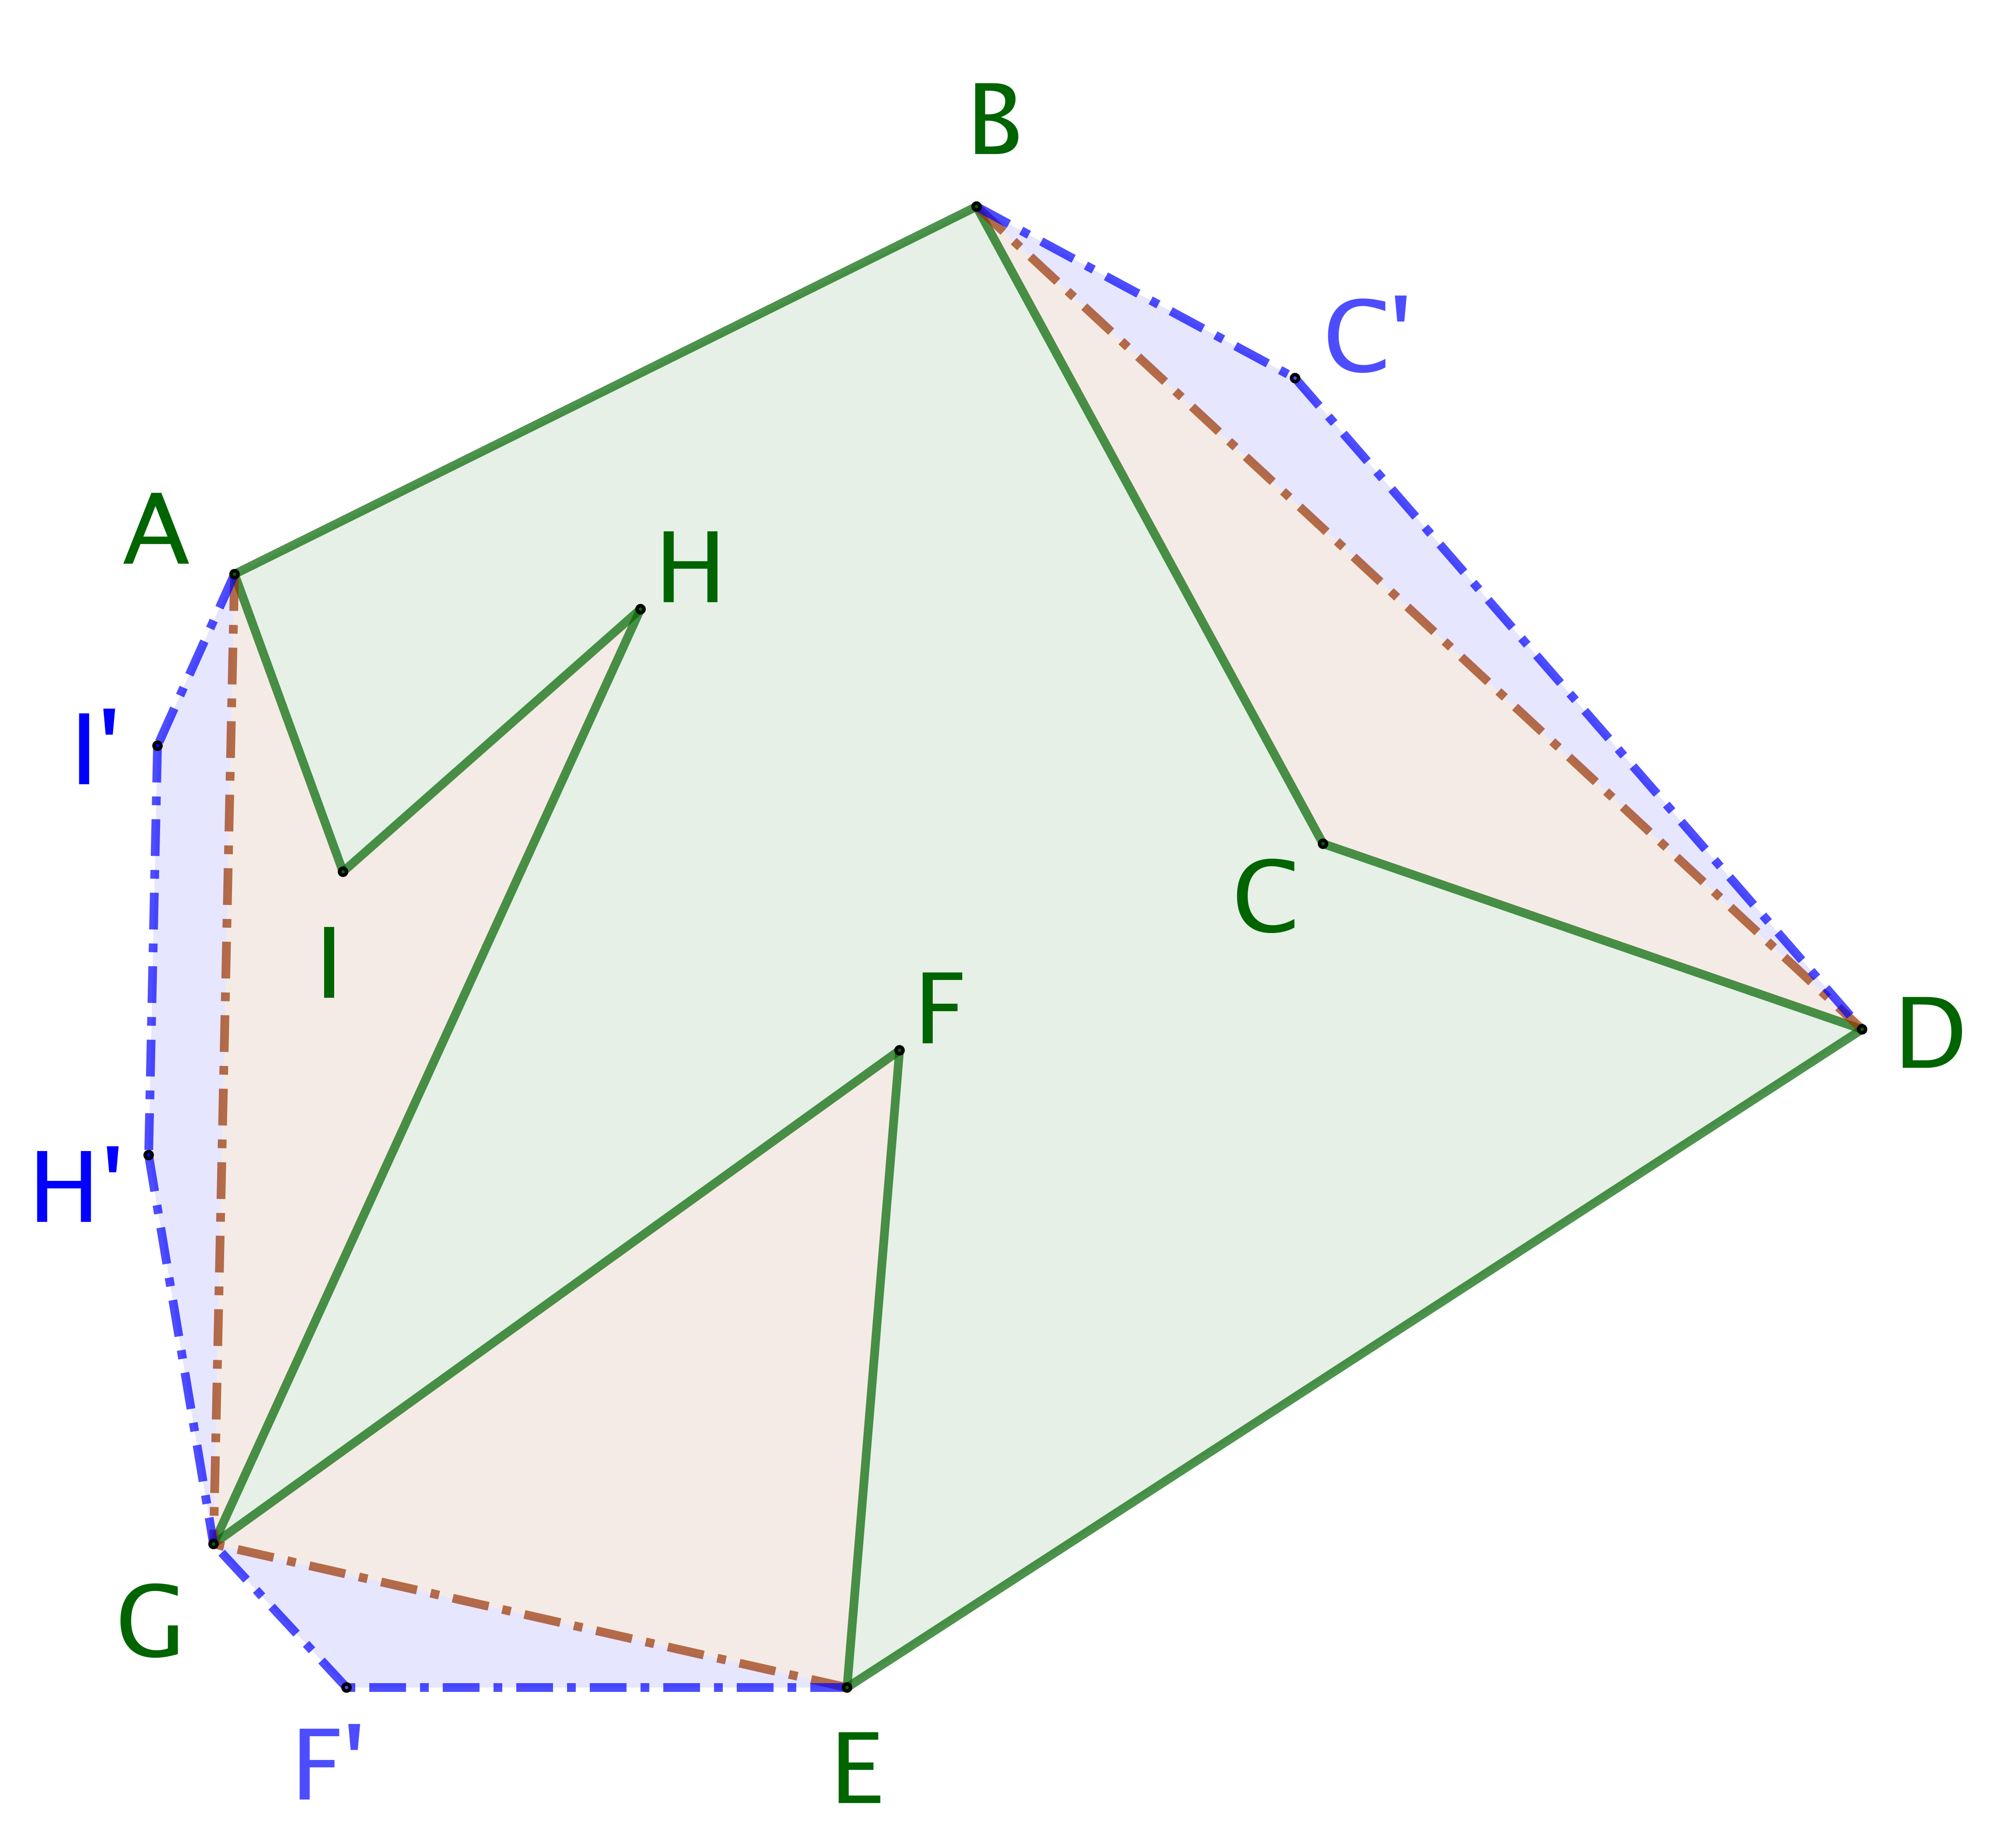
\includegraphics[scale=.4]{content/polygon/polygon-convex-hull-distortion.png}
	\end{center}

	XXX
	%
	\begin{itemize}
		\item XXX

		\item XXX

		\item XXX

		\item XXX
	\end{itemize}
\end{proof}


% ----------------------- %


\begin{fact}\label{iso-poly}
	Si un $n$-gone convexe $\setproba{P}$, de périmètre fixé $p$, n'est pas un $n$-isogone, alors on peut construire à partir de $\setproba{P}$ un $n$-isogone convexe $\setproba{P}^{\,\prime}$ tel que $\perim{\setproba{P}^{\,\prime}} = p$ et $\area{\setproba{P}^{\,\prime}} > \area{\setproba{P}}$.
\end{fact}


\begin{proof}
	XXX
\end{proof}


% ----------------------- %


Les faits \ref{conv-poly} et \ref{iso-poly} précédents permettent de se restreindre au cas des $n$-isogones convexes. Ceci nous amène au beau résultat suivant.

\begin{fact}\label{reg-poly}
	Si un $n$-isogone convexe $\setproba{P}$ de périmètre fixé $p$ possède au moins deux angles de mesures différentes, alors on peut construire à partir de $\setproba{P}$ un $n$-gone régulier $\setproba{P}^{\,\prime}$ tel que $\perim{\setproba{P}^{\,\prime}} = p$ et $\area{\setproba{P}^{\,\prime}} > \area{\setproba{P}}$.
\end{fact}


\begin{proof}
	XXX
\end{proof}


% ----------------------- %


\begin{fact}
	Soit $n \in \NN_{\geq3}$ un naturel fixé.
	Considérons tous les $n$-gones de périmètre fixé $p$. Parmi tous ces $n$-gones, un seul est d'aire maximale, c'est le $n$-gone régulier.
\end{fact}


\begin{proof}
	Tout a déjà été dit, car d'après les faits ci-dessus, un $n$-gone $\setproba{P}$ non régulier ne peut pas maximiser son aire à périmètre fixé, et par conséquent seul le $n$-gone régulier maximise l'aire à périmètre fixé. Chapeau bas, géométrie...
\end{proof}


\end{document}
